
% ------------------ DOCUMENT SETUP ------------------ 
% The document class defines the document type (report) and sets the font size (10pt)
\documentclass{report}

% Optional math commands from https://github.com/goodfeli/dlbook_notation.
%%%%% NEW MATH DEFINITIONS %%%%%

\usepackage{amsmath,amsfonts,bm}

% Mark sections of captions for referring to divisions of figures
\newcommand{\figleft}{{\em (Left)}}
\newcommand{\figcenter}{{\em (Center)}}
\newcommand{\figright}{{\em (Right)}}
\newcommand{\figtop}{{\em (Top)}}
\newcommand{\figbottom}{{\em (Bottom)}}
\newcommand{\captiona}{{\em (a)}}
\newcommand{\captionb}{{\em (b)}}
\newcommand{\captionc}{{\em (c)}}
\newcommand{\captiond}{{\em (d)}}

% Highlight a newly defined term
\newcommand{\newterm}[1]{{\bf #1}}


% Figure reference, lower-case.
\def\figref#1{figure~\ref{#1}}
% Figure reference, capital. For start of sentence
\def\Figref#1{Figure~\ref{#1}}
\def\twofigref#1#2{figures \ref{#1} and \ref{#2}}
\def\quadfigref#1#2#3#4{figures \ref{#1}, \ref{#2}, \ref{#3} and \ref{#4}}
% Section reference, lower-case.
\def\secref#1{section~\ref{#1}}
% Section reference, capital.
\def\Secref#1{Section~\ref{#1}}
% Reference to two sections.
\def\twosecrefs#1#2{sections \ref{#1} and \ref{#2}}
% Reference to three sections.
\def\secrefs#1#2#3{sections \ref{#1}, \ref{#2} and \ref{#3}}
% Reference to an equation, lower-case.
\def\eqref#1{equation~\ref{#1}}
% Reference to an equation, upper case
\def\Eqref#1{Equation~\ref{#1}}
% A raw reference to an equation---avoid using if possible
\def\plaineqref#1{\ref{#1}}
% Reference to a chapter, lower-case.
\def\chapref#1{chapter~\ref{#1}}
% Reference to an equation, upper case.
\def\Chapref#1{Chapter~\ref{#1}}
% Reference to a range of chapters
\def\rangechapref#1#2{chapters\ref{#1}--\ref{#2}}
% Reference to an algorithm, lower-case.
\def\algref#1{algorithm~\ref{#1}}
% Reference to an algorithm, upper case.
\def\Algref#1{Algorithm~\ref{#1}}
\def\twoalgref#1#2{algorithms \ref{#1} and \ref{#2}}
\def\Twoalgref#1#2{Algorithms \ref{#1} and \ref{#2}}
% Reference to a part, lower case
\def\partref#1{part~\ref{#1}}
% Reference to a part, upper case
\def\Partref#1{Part~\ref{#1}}
\def\twopartref#1#2{parts \ref{#1} and \ref{#2}}

\def\ceil#1{\lceil #1 \rceil}
\def\floor#1{\lfloor #1 \rfloor}
\def\1{\bm{1}}
\newcommand{\train}{\mathcal{D}}
\newcommand{\valid}{\mathcal{D_{\mathrm{valid}}}}
\newcommand{\test}{\mathcal{D_{\mathrm{test}}}}

\def\eps{{\epsilon}}


% Random variables
\def\reta{{\textnormal{$\eta$}}}
\def\ra{{\textnormal{a}}}
\def\rb{{\textnormal{b}}}
\def\rc{{\textnormal{c}}}
\def\rd{{\textnormal{d}}}
\def\re{{\textnormal{e}}}
\def\rf{{\textnormal{f}}}
\def\rg{{\textnormal{g}}}
\def\rh{{\textnormal{h}}}
\def\ri{{\textnormal{i}}}
\def\rj{{\textnormal{j}}}
\def\rk{{\textnormal{k}}}
\def\rl{{\textnormal{l}}}
% rm is already a command, just don't name any random variables m
\def\rn{{\textnormal{n}}}
\def\ro{{\textnormal{o}}}
\def\rp{{\textnormal{p}}}
\def\rq{{\textnormal{q}}}
\def\rr{{\textnormal{r}}}
\def\rs{{\textnormal{s}}}
\def\rt{{\textnormal{t}}}
\def\ru{{\textnormal{u}}}
\def\rv{{\textnormal{v}}}
\def\rw{{\textnormal{w}}}
\def\rx{{\textnormal{x}}}
\def\ry{{\textnormal{y}}}
\def\rz{{\textnormal{z}}}

% Random vectors
\def\rvepsilon{{\mathbf{\epsilon}}}
\def\rvtheta{{\mathbf{\theta}}}
\def\rva{{\mathbf{a}}}
\def\rvb{{\mathbf{b}}}
\def\rvc{{\mathbf{c}}}
\def\rvd{{\mathbf{d}}}
\def\rve{{\mathbf{e}}}
\def\rvf{{\mathbf{f}}}
\def\rvg{{\mathbf{g}}}
\def\rvh{{\mathbf{h}}}
\def\rvu{{\mathbf{i}}}
\def\rvj{{\mathbf{j}}}
\def\rvk{{\mathbf{k}}}
\def\rvl{{\mathbf{l}}}
\def\rvm{{\mathbf{m}}}
\def\rvn{{\mathbf{n}}}
\def\rvo{{\mathbf{o}}}
\def\rvp{{\mathbf{p}}}
\def\rvq{{\mathbf{q}}}
\def\rvr{{\mathbf{r}}}
\def\rvs{{\mathbf{s}}}
\def\rvt{{\mathbf{t}}}
\def\rvu{{\mathbf{u}}}
\def\rvv{{\mathbf{v}}}
\def\rvw{{\mathbf{w}}}
\def\rvx{{\mathbf{x}}}
\def\rvy{{\mathbf{y}}}
\def\rvz{{\mathbf{z}}}

% Elements of random vectors
\def\erva{{\textnormal{a}}}
\def\ervb{{\textnormal{b}}}
\def\ervc{{\textnormal{c}}}
\def\ervd{{\textnormal{d}}}
\def\erve{{\textnormal{e}}}
\def\ervf{{\textnormal{f}}}
\def\ervg{{\textnormal{g}}}
\def\ervh{{\textnormal{h}}}
\def\ervi{{\textnormal{i}}}
\def\ervj{{\textnormal{j}}}
\def\ervk{{\textnormal{k}}}
\def\ervl{{\textnormal{l}}}
\def\ervm{{\textnormal{m}}}
\def\ervn{{\textnormal{n}}}
\def\ervo{{\textnormal{o}}}
\def\ervp{{\textnormal{p}}}
\def\ervq{{\textnormal{q}}}
\def\ervr{{\textnormal{r}}}
\def\ervs{{\textnormal{s}}}
\def\ervt{{\textnormal{t}}}
\def\ervu{{\textnormal{u}}}
\def\ervv{{\textnormal{v}}}
\def\ervw{{\textnormal{w}}}
\def\ervx{{\textnormal{x}}}
\def\ervy{{\textnormal{y}}}
\def\ervz{{\textnormal{z}}}

% Random matrices
\def\rmA{{\mathbf{A}}}
\def\rmB{{\mathbf{B}}}
\def\rmC{{\mathbf{C}}}
\def\rmD{{\mathbf{D}}}
\def\rmE{{\mathbf{E}}}
\def\rmF{{\mathbf{F}}}
\def\rmG{{\mathbf{G}}}
\def\rmH{{\mathbf{H}}}
\def\rmI{{\mathbf{I}}}
\def\rmJ{{\mathbf{J}}}
\def\rmK{{\mathbf{K}}}
\def\rmL{{\mathbf{L}}}
\def\rmM{{\mathbf{M}}}
\def\rmN{{\mathbf{N}}}
\def\rmO{{\mathbf{O}}}
\def\rmP{{\mathbf{P}}}
\def\rmQ{{\mathbf{Q}}}
\def\rmR{{\mathbf{R}}}
\def\rmS{{\mathbf{S}}}
\def\rmT{{\mathbf{T}}}
\def\rmU{{\mathbf{U}}}
\def\rmV{{\mathbf{V}}}
\def\rmW{{\mathbf{W}}}
\def\rmX{{\mathbf{X}}}
\def\rmY{{\mathbf{Y}}}
\def\rmZ{{\mathbf{Z}}}

% Elements of random matrices
\def\ermA{{\textnormal{A}}}
\def\ermB{{\textnormal{B}}}
\def\ermC{{\textnormal{C}}}
\def\ermD{{\textnormal{D}}}
\def\ermE{{\textnormal{E}}}
\def\ermF{{\textnormal{F}}}
\def\ermG{{\textnormal{G}}}
\def\ermH{{\textnormal{H}}}
\def\ermI{{\textnormal{I}}}
\def\ermJ{{\textnormal{J}}}
\def\ermK{{\textnormal{K}}}
\def\ermL{{\textnormal{L}}}
\def\ermM{{\textnormal{M}}}
\def\ermN{{\textnormal{N}}}
\def\ermO{{\textnormal{O}}}
\def\ermP{{\textnormal{P}}}
\def\ermQ{{\textnormal{Q}}}
\def\ermR{{\textnormal{R}}}
\def\ermS{{\textnormal{S}}}
\def\ermT{{\textnormal{T}}}
\def\ermU{{\textnormal{U}}}
\def\ermV{{\textnormal{V}}}
\def\ermW{{\textnormal{W}}}
\def\ermX{{\textnormal{X}}}
\def\ermY{{\textnormal{Y}}}
\def\ermZ{{\textnormal{Z}}}

% Vectors
\def\vzero{{\bm{0}}}
\def\vone{{\bm{1}}}
\def\vmu{{\bm{\mu}}}
\def\vtheta{{\bm{\theta}}}
\def\va{{\bm{a}}}
\def\vb{{\bm{b}}}
\def\vc{{\bm{c}}}
\def\vd{{\bm{d}}}
\def\ve{{\bm{e}}}
\def\vf{{\bm{f}}}
\def\vg{{\bm{g}}}
\def\vh{{\bm{h}}}
\def\vi{{\bm{i}}}
\def\vj{{\bm{j}}}
\def\vk{{\bm{k}}}
\def\vl{{\bm{l}}}
\def\vm{{\bm{m}}}
\def\vn{{\bm{n}}}
\def\vo{{\bm{o}}}
\def\vp{{\bm{p}}}
\def\vq{{\bm{q}}}
\def\vr{{\bm{r}}}
\def\vs{{\bm{s}}}
\def\vt{{\bm{t}}}
\def\vu{{\bm{u}}}
\def\vv{{\bm{v}}}
\def\vw{{\bm{w}}}
\def\vx{{\bm{x}}}
\def\vy{{\bm{y}}}
\def\vz{{\bm{z}}}

% Elements of vectors
\def\evalpha{{\alpha}}
\def\evbeta{{\beta}}
\def\evepsilon{{\epsilon}}
\def\evlambda{{\lambda}}
\def\evomega{{\omega}}
\def\evmu{{\mu}}
\def\evpsi{{\psi}}
\def\evsigma{{\sigma}}
\def\evtheta{{\theta}}
\def\eva{{a}}
\def\evb{{b}}
\def\evc{{c}}
\def\evd{{d}}
\def\eve{{e}}
\def\evf{{f}}
\def\evg{{g}}
\def\evh{{h}}
\def\evi{{i}}
\def\evj{{j}}
\def\evk{{k}}
\def\evl{{l}}
\def\evm{{m}}
\def\evn{{n}}
\def\evo{{o}}
\def\evp{{p}}
\def\evq{{q}}
\def\evr{{r}}
\def\evs{{s}}
\def\evt{{t}}
\def\evu{{u}}
\def\evv{{v}}
\def\evw{{w}}
\def\evx{{x}}
\def\evy{{y}}
\def\evz{{z}}

% Matrix
\def\mA{{\bm{A}}}
\def\mB{{\bm{B}}}
\def\mC{{\bm{C}}}
\def\mD{{\bm{D}}}
\def\mE{{\bm{E}}}
\def\mF{{\bm{F}}}
\def\mG{{\bm{G}}}
\def\mH{{\bm{H}}}
\def\mI{{\bm{I}}}
\def\mJ{{\bm{J}}}
\def\mK{{\bm{K}}}
\def\mL{{\bm{L}}}
\def\mM{{\bm{M}}}
\def\mN{{\bm{N}}}
\def\mO{{\bm{O}}}
\def\mP{{\bm{P}}}
\def\mQ{{\bm{Q}}}
\def\mR{{\bm{R}}}
\def\mS{{\bm{S}}}
\def\mT{{\bm{T}}}
\def\mU{{\bm{U}}}
\def\mV{{\bm{V}}}
\def\mW{{\bm{W}}}
\def\mX{{\bm{X}}}
\def\mY{{\bm{Y}}}
\def\mZ{{\bm{Z}}}
\def\mBeta{{\bm{\beta}}}
\def\mPhi{{\bm{\Phi}}}
\def\mLambda{{\bm{\Lambda}}}
\def\mSigma{{\bm{\Sigma}}}

% Tensor
\DeclareMathAlphabet{\mathsfit}{\encodingdefault}{\sfdefault}{m}{sl}
\SetMathAlphabet{\mathsfit}{bold}{\encodingdefault}{\sfdefault}{bx}{n}
\newcommand{\tens}[1]{\bm{\mathsfit{#1}}}
\def\tA{{\tens{A}}}
\def\tB{{\tens{B}}}
\def\tC{{\tens{C}}}
\def\tD{{\tens{D}}}
\def\tE{{\tens{E}}}
\def\tF{{\tens{F}}}
\def\tG{{\tens{G}}}
\def\tH{{\tens{H}}}
\def\tI{{\tens{I}}}
\def\tJ{{\tens{J}}}
\def\tK{{\tens{K}}}
\def\tL{{\tens{L}}}
\def\tM{{\tens{M}}}
\def\tN{{\tens{N}}}
\def\tO{{\tens{O}}}
\def\tP{{\tens{P}}}
\def\tQ{{\tens{Q}}}
\def\tR{{\tens{R}}}
\def\tS{{\tens{S}}}
\def\tT{{\tens{T}}}
\def\tU{{\tens{U}}}
\def\tV{{\tens{V}}}
\def\tW{{\tens{W}}}
\def\tX{{\tens{X}}}
\def\tY{{\tens{Y}}}
\def\tZ{{\tens{Z}}}


% Graph
\def\gA{{\mathcal{A}}}
\def\gB{{\mathcal{B}}}
\def\gC{{\mathcal{C}}}
\def\gD{{\mathcal{D}}}
\def\gE{{\mathcal{E}}}
\def\gF{{\mathcal{F}}}
\def\gG{{\mathcal{G}}}
\def\gH{{\mathcal{H}}}
\def\gI{{\mathcal{I}}}
\def\gJ{{\mathcal{J}}}
\def\gK{{\mathcal{K}}}
\def\gL{{\mathcal{L}}}
\def\gM{{\mathcal{M}}}
\def\gN{{\mathcal{N}}}
\def\gO{{\mathcal{O}}}
\def\gP{{\mathcal{P}}}
\def\gQ{{\mathcal{Q}}}
\def\gR{{\mathcal{R}}}
\def\gS{{\mathcal{S}}}
\def\gT{{\mathcal{T}}}
\def\gU{{\mathcal{U}}}
\def\gV{{\mathcal{V}}}
\def\gW{{\mathcal{W}}}
\def\gX{{\mathcal{X}}}
\def\gY{{\mathcal{Y}}}
\def\gZ{{\mathcal{Z}}}

% Sets
\def\sA{{\mathbb{A}}}
\def\sB{{\mathbb{B}}}
\def\sC{{\mathbb{C}}}
\def\sD{{\mathbb{D}}}
% Don't use a set called E, because this would be the same as our symbol
% for expectation.
\def\sF{{\mathbb{F}}}
\def\sG{{\mathbb{G}}}
\def\sH{{\mathbb{H}}}
\def\sI{{\mathbb{I}}}
\def\sJ{{\mathbb{J}}}
\def\sK{{\mathbb{K}}}
\def\sL{{\mathbb{L}}}
\def\sM{{\mathbb{M}}}
\def\sN{{\mathbb{N}}}
\def\sO{{\mathbb{O}}}
\def\sP{{\mathbb{P}}}
\def\sQ{{\mathbb{Q}}}
\def\sR{{\mathbb{R}}}
\def\sS{{\mathbb{S}}}
\def\sT{{\mathbb{T}}}
\def\sU{{\mathbb{U}}}
\def\sV{{\mathbb{V}}}
\def\sW{{\mathbb{W}}}
\def\sX{{\mathbb{X}}}
\def\sY{{\mathbb{Y}}}
\def\sZ{{\mathbb{Z}}}

% Entries of a matrix
\def\emLambda{{\Lambda}}
\def\emA{{A}}
\def\emB{{B}}
\def\emC{{C}}
\def\emD{{D}}
\def\emE{{E}}
\def\emF{{F}}
\def\emG{{G}}
\def\emH{{H}}
\def\emI{{I}}
\def\emJ{{J}}
\def\emK{{K}}
\def\emL{{L}}
\def\emM{{M}}
\def\emN{{N}}
\def\emO{{O}}
\def\emP{{P}}
\def\emQ{{Q}}
\def\emR{{R}}
\def\emS{{S}}
\def\emT{{T}}
\def\emU{{U}}
\def\emV{{V}}
\def\emW{{W}}
\def\emX{{X}}
\def\emY{{Y}}
\def\emZ{{Z}}
\def\emSigma{{\Sigma}}

% entries of a tensor
% Same font as tensor, without \bm wrapper
\newcommand{\etens}[1]{\mathsfit{#1}}
\def\etLambda{{\etens{\Lambda}}}
\def\etA{{\etens{A}}}
\def\etB{{\etens{B}}}
\def\etC{{\etens{C}}}
\def\etD{{\etens{D}}}
\def\etE{{\etens{E}}}
\def\etF{{\etens{F}}}
\def\etG{{\etens{G}}}
\def\etH{{\etens{H}}}
\def\etI{{\etens{I}}}
\def\etJ{{\etens{J}}}
\def\etK{{\etens{K}}}
\def\etL{{\etens{L}}}
\def\etM{{\etens{M}}}
\def\etN{{\etens{N}}}
\def\etO{{\etens{O}}}
\def\etP{{\etens{P}}}
\def\etQ{{\etens{Q}}}
\def\etR{{\etens{R}}}
\def\etS{{\etens{S}}}
\def\etT{{\etens{T}}}
\def\etU{{\etens{U}}}
\def\etV{{\etens{V}}}
\def\etW{{\etens{W}}}
\def\etX{{\etens{X}}}
\def\etY{{\etens{Y}}}
\def\etZ{{\etens{Z}}}

% The true underlying data generating distribution
\newcommand{\pdata}{p_{\rm{data}}}
% The empirical distribution defined by the training set
\newcommand{\ptrain}{\hat{p}_{\rm{data}}}
\newcommand{\Ptrain}{\hat{P}_{\rm{data}}}
% The model distribution
\newcommand{\pmodel}{p_{\rm{model}}}
\newcommand{\Pmodel}{P_{\rm{model}}}
\newcommand{\ptildemodel}{\tilde{p}_{\rm{model}}}
% Stochastic autoencoder distributions
\newcommand{\pencode}{p_{\rm{encoder}}}
\newcommand{\pdecode}{p_{\rm{decoder}}}
\newcommand{\precons}{p_{\rm{reconstruct}}}

\newcommand{\laplace}{\mathrm{Laplace}} % Laplace distribution

\newcommand{\E}{\mathbb{E}}
\newcommand{\Ls}{\mathcal{L}}
\newcommand{\R}{\mathbb{R}}
\newcommand{\emp}{\tilde{p}}
\newcommand{\lr}{\alpha}
\newcommand{\reg}{\lambda}
\newcommand{\rect}{\mathrm{rectifier}}
\newcommand{\softmax}{\mathrm{softmax}}
\newcommand{\sigmoid}{\sigma}
\newcommand{\softplus}{\zeta}
\newcommand{\KL}{D_{\mathrm{KL}}}
\newcommand{\Var}{\mathrm{Var}}
\newcommand{\standarderror}{\mathrm{SE}}
\newcommand{\Cov}{\mathrm{Cov}}
% Wolfram Mathworld says $L^2$ is for function spaces and $\ell^2$ is for vectors
% But then they seem to use $L^2$ for vectors throughout the site, and so does
% wikipedia.
\newcommand{\normlzero}{L^0}
\newcommand{\normlone}{L^1}
\newcommand{\normltwo}{L^2}
\newcommand{\normlp}{L^p}
\newcommand{\normmax}{L^\infty}

\newcommand{\parents}{Pa} % See usage in notation.tex. Chosen to match Daphne's book.

\DeclareMathOperator*{\argmax}{arg\,max}
\DeclareMathOperator*{\argmin}{arg\,min}

\DeclareMathOperator{\sign}{sign}
\DeclareMathOperator{\Tr}{Tr}
\let\ab\allowbreak

\DeclareMathSymbol{\shortminus}{\mathbin}{AMSa}{"39}
\newcommand{\ppart}[1]{\textcolor{violet}{\max\Bigl(}{#1}\textcolor{violet}{,0\Bigr)}}
% bbm for indicator
\usepackage{bbm}
\newcommand{\ind}[1]{\mathbbm{1}_{\{{#1}\}}}
\newcommand{\ones}[1]{\mathrm{1}_{{#1}}}
\newcommand{\order}[1]{\mathcal{O}\left({#1}\right)}
% mathtools for defeq and eqdef
\usepackage{mathtools}
\newcommand{\defeq}{\vcentcolon=}
\newcommand{\eqdef}{=\vcentcolon}
% xfrac
\usepackage{xfrac}
\newcommand{\mhalf}{{\shortminus \sfrac{1}{2}}}
\newcommand{\half}{{\sfrac{1}{2}}}
\DeclarePairedDelimiter{\norm}{\lVert}{\rVert}
\newcommand{\tr}{\operatorname{trace}}
\newcommand{\diag}{\operatorname{diag}}
%\newcommand{\cspan}{{\operatorname{span}}}
\newcommand{\cspan}[1]{{\operatorname{span}\{{#1}\}}}
\newcommand{\PD}[1]{\mathbf{S}^{#1}_{++}}
\newcommand{\PSD}[1]{\mathbf{S}^{#1}_{+}}

\newcommand{\CCA}{\operatorname{CCA}}
\newcommand{\MCCA}{\operatorname{MCCA}}
\newcommand{\Corr}{\operatorname{Corr}}
\newcommand{\empCov}{\widehat{\Cov}}
\newcommand{\empVar}{\widehat{\Var}}
\newcommand{\empCorr}{\widehat{\Corr}}
\newcommand{\bGaminds}[1]{\textcolor{blue}{\Gamma_{#1}}}
\newcommand{\bGam}{\textcolor{blue}{\Gamma}}
\newcommand{\Sigxx}{\Sigma_{xx}}
\newcommand{\Sigxy}{\Sigma_{xy}}
\newcommand{\Sigyx}{\Sigma_{yx}}
\newcommand{\Sigyy}{\Sigma_{yy}}

\newcommand{\tilU}{\Tilde{U}}
\newcommand{\tilV}{\Tilde{V}}
\newcommand{\tilW}{\Tilde{W}}

\newcommand{\X}{\mathbf{X}}
\newcommand{\Y}{\mathbf{Y}}
\newcommand{\Z}{\mathbf{Z}}
\newcommand{\Xb}{\mathbf{X}^{(b)}}
\newcommand{\Yb}{\mathbf{Y}^{(b)}}
\newcommand{\sps}[1]{^{(#1)}} % convenient super scripts
\newcommand{\spsT}[1]{^{(#1)\,T}}
% \newcommand{\Xs}[1]{X^{({#1})}}
% \newcommand{\Zs}[1]{Z^{({#1})}}
\newcommand{\ninv}{\tfrac{1}{N}}

% Loss functions specific for this paper
\newcommand{\LBT}{\mathcal{L}_\text{BT}}
\newcommand{\LVR}{\mathcal{L}_\text{VR}}
\newcommand{\barLVR}{\bar{\mathcal{L}}_\text{VR}}
\newcommand{\barLBT}{\bar{\mathcal{L}}_\text{BT}}
\newcommand{\LEY}{\mathcal{L}_\text{EY}}
\newcommand{\LEYGEP}{\mathcal{L}_\text{EY-GEP}}
\newcommand{\empLEY}{\hat{\mathcal{L}}_\text{EY}}
\newcommand{\empLBT}{\hat{\mathcal{L}}_\text{BT}}
\newcommand{\empLVR}{\hat{\mathcal{L}}_\text{VR}}


% conditional expectations from
% https://tex.stackexchange.com/questions/187162/vertical-bar-for-absolute-value-and-conditional-expectation/187363#187363
% thank you to egreg!
% then augmented with chatGPT to allow subscripts also
% expect* gives automatic scaling, but warned to use sparingly

\NewDocumentCommand{\expect}{e{^}e{_} s o >{\SplitArgument{1}{|}}m }{%
  \mathbb{E}%     the expectation operator
  \IfValueT{#1}{^{#1}}% previously had {\!} to add thin negative spacing before the superscript
  \IfValueT{#2}{_{#2}}% previously had {\!} add thin negative spacing beforethe subscript
  \IfBooleanTF{#3}{% *-variant for automatic scaling
    \expectarg*{\expectvar#5}%
  }{% no *-variant
    \IfNoValueTF{#4}{% no optional argument for custom size
      \expectarg{\expectvar#5}%
    }{% optional argument for custom size
      \expectarg[#4]{\expectvar#5}%
    }%
  }%
}
\NewDocumentCommand{\expectvar}{mm}{%
  #1\IfValueT{#2}{\nonscript\;\delimsize\vert\nonscript\;#2}%
}
\DeclarePairedDelimiterX{\expectarg}[1]{[}{]}{#1}


\author{James Chapman}

% Inputs the Document Packages
% ------------------ PACKAGES ------------------ 

% Packages add extra commands and features to your LaTeX document. 
% Here are some of the most common packages for a thesis document.

% Floating environments for figures and tables
\usepackage{float}

% Color support
\usepackage{color}

% Epigraphs
\usepackage{epigraph}

% Color support for tables
\usepackage[table,xcdraw]{xcolor}

% Mathematical typesetting
\usepackage{amsthm}

% Theorem environments
\newtheorem{corollary}{Corollary}[section]
\newtheorem{definition}{Definition}[section]
\newtheorem{theorem}{Theorem}[section]
\newtheorem{lemma}{Lemma}[section]
\newtheorem{proposition}{Proposition}[section]
\newtheorem{example}{Example}[section]

% Remark environment
\theoremstyle{remark}
\newtheorem{remark}{Remark}

% Restatable theorems
\usepackage{thmtools}
\usepackage{thm-restate}
\declaretheorem[name=Proposition,numberwithin=section]{proprep}
\newtheorem{thm}{Theorem}

% Algorithms
\usepackage[ruled,vlined]{algorithm2e}
\usepackage{algorithmic}

% Vector arrows
\usepackage{esvect}

% TikZ for diagrams
\usepackage{tikz}
\usetikzlibrary{patterns, bayesnet, arrows, backgrounds}

% Hyperlinks
\usepackage{hyperref}
\hypersetup{
    citecolor = blue
}

% Multi-row tables
\usepackage{multirow}

% Appendices
\usepackage[toc,page]{appendix}

% Captioning figures and tables
\usepackage[format=hang,font=normalsize,labelfont=bf,labelsep=colon,singlelinecheck=off, justification=centering]{caption}
\usepackage{subcaption}

% Long tables
\usepackage{longtable}

% Glossaries and acronyms
\usepackage[acronym]{glossaries}

% Font settings
\usepackage[scaled]{helvet}
\usepackage[T1]{fontenc}
\renewcommand\familydefault{\sfdefault}

% Input encoding
\usepackage[utf8]{inputenc}

% Empty pages
\usepackage{emptypage}

% Importing files
\usepackage{import}

% Table of Contents customization
\usepackage{tocloft}

% Title customization
\usepackage{titlesec}

% Table of Contents title customization
\usepackage{titletoc}

% Alternative implementations for LaTeX commands
\usepackage{etoolbox}

% Header and footer control
\usepackage{fancyhdr} 

% Typography enhancements
\usepackage{microtype}

% PDF bookmarks
\usepackage{bookmark}

% Units and symbols
\usepackage{gensymb}
\usepackage{textcomp}

% Bibliography
\usepackage[natbib,style=authoryear,natbib=true]{biblatex}
\addbibresource{publications.bib} % Add the .bib file that contains the references
\addbibresource{References.bib} % Add the .bib file that contains the references

% Sample text
\usepackage{blindtext}

% Tables
\usepackage{booktabs}

% Code listings
\usepackage{listings}
\usepackage{minted}

% Math symbols
\usepackage{amsmath,amsfonts,bm}
\usepackage{amssymb}

% Clever referencing
\usepackage[capitalize,noabbrev]{cleveref}

% Graphics
\usepackage{graphicx}
\usepackage{svg}

% Restating theorems
\usepackage{thm-restate}

% Line spacing control
\usepackage{setspace}

% Mini table of contents
\usepackage{minitoc} 

% Mini TOC font settings
\renewcommand{\mtifont}{\large\sffamily}
\renewcommand{\mtcfont}{\small\sffamily}
\renewcommand{\mtcSfont}{\small\sffamily}
\renewcommand{\mtcSSfont}{\small\sffamily}
\renewcommand{\mtcSSSfont}{\small\sffamily}

% Add to table of contents
\newcommand\addtotoc[1]{
  \refstepcounter{dummy}
  \addcontentsline{toc}{chapter}{#1}
}


% Controls how many subsections the document can take
%  and how many of those will get put into the contents pages.
\setcounter{secnumdepth}{3}
\setcounter{tocdepth}{2}

% Places a dot after Chapter/Section/Subsection number in Table of Contents
\renewcommand{\cftchapaftersnum}{.}
\renewcommand{\cftsecaftersnum}{.}
\renewcommand{\cftsubsecaftersnum}{.}

%  Customize Dot spacing in Table of Contents/List of Figures/Tables
\renewcommand{\cftdotsep}{0.3}

% Numeration Type for Chapters and Sections (Roman I, II, II / Arabic 1, 2, 3)
\renewcommand\thechapter{\Roman{chapter}}
\renewcommand\thesection{\arabic{section}}

% Formatting Table of Contents/Lists titles
\renewcommand{\contentsname}{\normalfont\bfseries\LARGE{CONTENTS}}
\renewcommand{\listfigurename}{\normalfont\bfseries\LARGE{LIST OF FIGURES}}
\renewcommand{\listtablename}{\normalfont\bfseries\LARGE{LIST OF TABLES}}


% HEADER AND FOOTER
\pagestyle{fancy}  % Set Page Style (Header and Footer Style)
\fancyhf{}  % Clears the header and footer (from the default info)

% Header
\renewcommand{\headrulewidth}{0pt}  % Removes the default Horizontal Line in Header
\fancyhead[L]{James Chapman}
\fancyhead[R]{January 2022}

% Footer
\fancyfoot[C]{\thepage} % Page Number

% Change figure numbering per section
\numberwithin{figure}{chapter}
\numberwithin{table}{section}






%  -------------------------------------------------
%  --------- The document starts from here --------- 
%  -------------------------------------------------

\begin{document}

% ------------------  TITLE PAGE -------------------
\begin{titlepage}
\begin{center}
    % Title
    {\LARGE\textbf{Towards Scalable, Flexible, and Interpretable Self-Supervised Learning from Multiview Biomedical Data}
\author{James Chapman\\
    % Subtitle
    \\}}

    \vspace{0.8cm}
    by\\
    \vspace{0.8cm}

    % Author
    {\LARGE\textbf{James Chapman\\}}
    % Date
    \vspace{1.5cm}
    {\LARGE\textbf{January 2022}}

    \vfill

    \textbf{\setstretch{2.0}       
    Upgrade Report\\
    \vspace{1cm}
    i4health CDT\\
    University College London\\}

    \vspace{2cm}
\end{center}
\end{titlepage}

\onehalfspacing

% ----------------------  ABSTRACT -----------------------
\newpage
\chapter*{Abstract} % the Asterix (*) indicates that this section will be added to the table of contents but no number will be present beside it.
% \addcontentsline{toc}{chapter}{Abstract}

Biomedical data are essential for advancing our knowledge and practice of medicine and healthcare. However, biomedical data are also challenging to analyze due to their complexity, heterogeneity, high-dimensionality, and scarcity of labels. To overcome these challenges, self-supervised learning (SSL) has emerged as a promising paradigm for learning from unlabeled data by leveraging inherent structures or patterns in the data. SSL methods can exploit different forms of supervision signals derived from the data itself, such as contrastive learning, reconstruction, prediction, or clustering. SSL methods can also benefit from deep neural networks that can learn expressive and flexible representations from complex and high-dimensional data.

In this thesis, we focus on a specific type of SSL problem, namely multiview SSL, where data are represented by multiple distinct feature groups or modalities that describe the same phenomenon or entity. Each feature group or modality is referred to as a view, and different views may provide complementary or redundant information. Multiview SSL aims to learn useful representations from multiview data by exploiting the inherent structures or patterns across views. Multiview SSL has a wide range of applications in biomedical domains, such as integrating multiple types of genomic data for disease diagnosis or prognosis, generating natural language descriptions from brain images, and understanding human behaviors during social interactions based on multimodal signals.

In this thesis, we propose novel approaches to multiview SSL that are scalable, flexible, and interpretable. We address the following research questions:How can we reformulate classical subspace learning methods as unconstrained optimization problems that can be solved by gradient descent? How can we extend classical subspace learning methods to nonlinear functions using deep neural networks? How can we incorporate different forms of regularization or prior knowledge into subspace learning methods to improve their quality or robustness?

To answer these questions, we develop novel methods for multiview subspace learning that leverage mathematical optimization techniques, deep neural networks, regularization techniques. We evaluate our methods on various real-world biomedical datasets and demonstrate their effectiveness and advantages over existing methods.

% ----------------------  IMPACT STATEMENT -----------------------
\newpage
\chapter*{Impact Statement} % the Asterix (*) indicates that this section will be added to the table of contents but no number will be present beside it.
% \addcontentsline{toc}{chapter}{Impact}

This thesis contributes to the advancement of machine learning and biomedical data analysis by developing novel methods for multiview self-supervised learning that are scalable, flexible, and interpretable. The proposed methods can help researchers and practitioners to analyze complex and high-dimensional biomedical data more efficiently and effectively, and to discover new insights and opportunities for improving health outcomes. The proposed methods can also be applied to other domains where multiview data are available or desirable, such as natural language processing, computer vision, multimedia analysis, and social network analysis. This thesis also provides a valuable reference for future research on multiview self-supervised learning and related topics.

% -----------------  ACKNOWLEDGEMENTS  -------------------
\newpage
\chapter*{Acknowledgements}

Thanks to my supervisors, Professor Janaina Mourao-Miranda and Professor John Shawe-Taylor, for their contributions. 
I am very grateful to the EPSRC UCL Centre for Doctoral Training (CDT) in Intelligent, Integrated Imaging in Healthcare (i4Health) and NIHR UCLH Biomedical
Research Centre for funding this research.
Thanks to G-Research for funding my trip to NeurIPS 2023 to present my work.

To my incredible friends and coauthors, Ana and Lennie, I couldn't have done this without you. Ana, you kept our paper alive when I had given up on it (as well as the PhD). Lennie, your brutal honesty about the work being rubbish made it infinitely better. Florence, I was honored to be included on Fusili and for the hard lessons you taught me in marketing.

To members of the Machine Learning for Neuroimaging group at UCL, the Centre for Medical Imaging Computing, and all of the friends from 90 High Holborn.
Cemre, we could and should have done so much more together, but I am grateful for your advice before you left. 
Agoston, I was inspired your immense knowledge of the field.
Rick, you were everpresent in the office whenever the pandemic allowed, and I am grateful for your advice.
To the Mojo Dojo Casa House, thank you for making my NeurIPS 2023 experience unforgettable.

To the boat clubs of University College London, University of London, and Vesta Rowing Club who have provided an outlet that gave me a sense of progress, purpose, and community, even when academia had me down. Thanks also to all of the friends from the $\frac{1}{2}$ pint club, M\&G, and otherwise who have listened to me complain about my PhD.

Thanks to my mum and dad, obviously this has been a bit of a rollercoaster, but I am grateful for every helpful conversation we have had. And finally with love to Rebecca. On about our third date, you came to visit Leamington Spa to scout out PhDs. You have experienced every good and bad moment. You have been proud of me. We got through this together and we will get through the next thing together too.




% -------------------  LIST OF Publication ---------------------
% \newpage
% \chapter*{Publications}
\label{Publications}




% -------------------  LIST OF FIGURES --------------------
\newpage 
% {\let\oldnumberline\numberline       % Uncomment to add the word 'Figure' to figure number in List of Figures
%\renewcommand{\numberline}{\figurename~\oldnumberline}  
\listoffigures%
% \addcontentsline{toc}{chapter}{List of Figures} % Add List of figures into contents without any numeration 

% -------------------  LIST OF TABLES ---------------------
\newpage
\listoftables 
% \addcontentsline{toc}{chapter}{List of Tables} % Add List of tables into contents without any numeration 

% -------------------  ACRONYMS ---------------------
\newpage

% -------------------  NOTATION ---------------------
\newpage


% ------------------  TABLE OF CONTENTS --------------------
\dominitoc% Initialization
\tableofcontents 


%\textbf{Keywords:} Machine Learning, Neuroimaging, Canonical Correlation Analysis



% ------------------  CHAPTER START  --------------------
\chapter{Introduction}\label{Introduction}
\minitoc
\section{Setting the Stage: Biomedical Data and The Need for Effective Analytical Techniques}

The advent of modern technologies in biomedical research has led to an unprecedented surge in the quantity and complexity of data generated. From genomic sequences and proteomic profiles to neuroimaging and electronic health records, these multilayered datasets are a treasure trove of potential insights into disease processes and patient health. The ultimate goal of deciphering these intricate datasets is to enhance patient stratification processes, enabling a move towards personalised, precision healthcare. However, the analytical challenges posed by the scale, complexity, and heterogeneity of these datasets, coupled with the scarcity of labelled data, are significant.

In light of these challenges, this thesis proposes new methodologies based on unsupervised and self-supervised learning to extract meaningful information from these large, unlabelled, and complex biomedical datasets. It presents a specific focus on Canonical Correlation Analysis (CCA), a widely used technique in the area of multi-view self-supervised learning (SSL), which, while powerful, comes with its own set of limitations when dealing with large-scale biomedical data.

\section{Problem Statement: The Need for Scalable, Flexible, and Interpretable Multiview SSL Methods}

Despite the advantages offered by multiview SSL methods in handling complex and high-dimensional biomedical data, the existing methodologies face substantial limitations, particularly concerning scalability, flexibility, and interpretability. The computational costs of traditional algorithms for solving CCA and other generalized eigenvalue problems are prohibitive when dealing with large-scale datasets. This limitation directly impacts their scalability and applicability to modern biomedical datasets. Moreover, the inherent inflexibility of traditional methods fails to capture the nonlinear relationships often present in biomedical data.

\section{Thesis Structure and Contributions}

This thesis is structured as follows:

In Chapter 2, we will provide an in-depth literature review on multiview learning and self-supervised learning techniques, establishing a foundational understanding of these methodologies in the context of biomedical data.

In Chapter 3, we propose a novel formulation for CCA, introducing an approach to solve it by gradient descent. This methodology allows for scalable solutions by enabling stochastic gradient descent, thus overcoming the limitations of traditional full-batch algorithms.

In Chapter 4, we introduce regularization via proximal gradient descent into our framework. This addition allows us to incorporate structured priors into our model, improving the interpretability of our findings, and enhancing their relevance to the biomedical context.

In Chapter 5, we show our approach can be extended to Deep CCA and Self-Supervised Learning more generally. While the sample sizes in biomedical research are still too small to apply these methods, we lay the groundwork for their potential incorporation into our framework in the future.

In Chapter 6, we present CCA-Zoo, a Python package for CCA and multiview learning, which implements the methodologies proposed in this thesis. We show how this work filled a gap in the Python ecostystem, and how it will facilitate the adoption of these methods in the biomedical community.

In Chapter 7, we discuss the implications, challenges, and limitations of our work, and how they can be addressed in future research.

The main contributions of this thesis are:

\begin{itemize}
    \item The introduction of a new formulation for CCA and generalized eigenvalue problems which can be solved via gradient descent, enabling the scaling of these methods to much larger datasets.
    \item The integration of regularization into the proposed framework using proximal gradient descent, enabling the inclusion of structured priors and improving the interpretability of the findings.
    \item Laying the groundwork for the potential incorporation of deep learning methods into the framework when the sample size permits, enabling the capture of non-linear associations in the data.
    \item
\end{itemize}

Through these contributions, this thesis strives to bridge the gap between the potential of large-scale, complex biomedical data and the capabilities of existing analytical methodologies, bringing us one step closer to truly personalised medicine.

\chapter{Background: Multiview Machine Learning: Concepts, Methods, and Limitations}
\label{chap:background}
\minitoc

\section{Machine Learning}
Machine learning is a subfield of computer science that automates the process of data analysis, enabling systems to learn from data and make decisions without being explicitly programmed.
It is a cornerstone of modern artificial intelligence, offering a set of tools that extends far beyond traditional statistical methods.
These automated methods are used in a myriad of applications, from filtering spam emails to making medical diagnoses and powering self-driving cars.

This field is generally divided into three primary categories: supervised, unsupervised, and reinforcement learning.
Each of these paradigms is suited to a different type of problem, and the choice of approach often depends on the type and amount of data available.
This thesis will focus on a specialized area of machine learning known as `multiview machine learning," which deals with data sets that contain multiple types or `views" of information.

\subsection{Supervised Learning}

Supervised learning is a machine learning paradigm where the algorithm learns from labeled training data, and makes predictions or decisions based on that data.
This type of learning allows for the mapping of input data to output labels, essentially using annotated examples to discern how to generalize to unseen data.
A classic example of supervised learning is a spam email filter, where a model is trained on a dataset of emails labeled as 'spam' or 'not spam', and the task is to classify new, incoming emails into one of these categories.

The primary components of supervised learning include a set of input-output pairs known as the training set.
The goal is to find a function that approximates the relationship between the corresponding input and output variables.
This function is then applied to new, unseen data to make predictions or decisions.

\subsection{Unsupervised Learning}

Unsupervised learning methods learn a mapping from inputs to outputs without any training targets.
Unsupervised learning methods can be used to learn representations of the data that can be used for downstream tasks such as classification or regression.
They can also be used as a way to discover relationships between the data, such as understanding the underlying structure of the data or finding correlations between different modalities of data.
Some generative models can also be used to generate new data with similar characteristics to the training data.

Perhaps the most well-known example of unsupervised learning is principal components analysis (PCA), which learns a mapping from inputs to outputs based on the directions of maximum variance in the data.
PCA can be used to learn a low-dimensional representation of the data that captures the most variance in the data.

\subsection{Self-Supervised Learning}

Self-supervised learning methods learn a mapping from inputs to outputs based on a training signal that is derived from the data itself.
The transformer model behind the success of many Large Language Models (LLMs) such as BERT \cite{devlin2018bert} and GPT-3 \cite{brown2020language} is trained using a self-supervised learning method called masked language modelling.
In masked language modelling, the model is trained to predict a masked word in a sentence based on the other words in the sentence.
Of closer relevance to this PhD thesis is work on self-supervised learning for computer vision tasks.
In these methods, the model is trained to predict a patch of an image based on the other patches in the image.

Like unsupervised learning methods, self-supervised learning methods can be used to learn representations of the data that can be used for downstream tasks such as classification or regression.

\subsection{Multiview Machine Learning}

Throughout this report we will refer to different modalities of data for the same subject as different `views', consistent with the literature\cite{sun2013survey}.
Multiview machine learning is a branch of machine learning that deals with data that have multiple sources or modalities that describe the same phenomenon or entity.
For example, a person can be represented by their face image, voice, text, and gesture.
Each source or modality is referred to as a view, and different views may provide complementary or redundant information.

Multiview learning methods can be used to generate robust low-dimensional representations for a downstream task such as classification or regression, or to discover relationships between views such as correlation or even causation.
They been widely applied across a range of fields such as neuroimaging\cite{Krishnan2011}, finance\cite{cassel2000measurement}, Imaging Genetics\cite{Hansen2021}, to find associations between views in large datasets.

Multiview machine learning methods can be interpreted as either unsupervised or self-supervised depending on the underlying assumptions about their data-generating process.
Specifically, the presence of a shared latent variable can influence how we categorize these methods.
This interpretation will have important implications for the methods that we consider in this thesis.

\subsection{Unsupervised Multiview Machine Learning}
In unsupervised multiview machine learning, the focus is typically on finding a shared representation that captures the essence of different views without making any assumptions about the nature of these views.
The main idea here is that each view provides a different `angle' on the same object or phenomenon, but there is no explicit modeling of a shared latent variable that generates these views.
Methods such as Canonical Correlation Analysis (CCA) aim to maximize the correlation between the different views in a
common space but do not inherently posit that these views come from a single latent source.

\subsection{Self-Supervised Multiview Machine Learning}
Self-supervised multiview machine learning, on the other hand, often assumes that the different views are generated from a common latent variable.
In this sense, one can argue that the task of learning from multiview data becomes a form of self-supervised learning.

It is important to note that the distinction between unsupervised and self-supervised learning is not always clear-cut.
In particular, we will argue that a number of classical subspace learning algorithms including Canonical Correlation
Analysis (CCA) can be interpreted as both an unsupervised (learning associations between views) and a self-supervised (where the derived target is the subject) method depending on the context.



\section{Learning Representations}

Suppose we have a sequence of vector-valued random variables $X^{(i)} \in \R^{D_i}$ for $i \in \{1, \dots, I \}$
We want to learn meaningful $K$-dimensional representations
\begin{equation}\label{eq:general-form-of-representations}
    Z\sps{i} = f\sps{i}( X\sps{i}; \theta\sps{i}).
\end{equation}
For convenience, define $D = \sum_{i=1}^I D_i$ and $\theta = \left(\theta\sps{i}\right)_{i=1}^I$.
Without loss of generality take $D_1 \geq D_2 \geq \cdots \geq D_I$.
We will consistently use the subscripts $i,j \in [I]$ for views;
$d \in [D_i]$ for dimensions of input variables;
and $l,k \in [K]$ for dimensions of representations - i.e. to subscript dimensions of $Z\sps{i}, f\sps{i}$.
Later on we will introduce total number of samples $N$.

\subsection{Principal Components Analysis}

Principal Components Analysis (PCA)\cite{hotelling1933analysis} is a classical method in unsupervised machine learning for representation learning.
It is widely used for dimensionality reduction and feature extraction.
The primary goal of PCA is to transform the original high-dimensional data into a new coordinate system defined by orthogonal axes, capturing the most relevant aspects of the data.

\paragraph{Mathematical Formalism} In PCA, the representations are constrained to be linear transformations of the form:
\begin{equation}\label{eq:pca-linear-function-def}
    Z_k = X u_k,
\end{equation}
where $u_k$ are the orthonormal basis vectors:
\begin{equation}\label{eq:pca-orthonormality-constraint}
    u_k^\top u_l = \delta_{kl}.
\end{equation}

In this report, we will typically refer to $u_k$ as \textbf{weights}, $Z_k = X u_k$ as \textbf{representations},\textbf{latent
dimensions}, or \textbf{scores} depending on the context. We will sometimes consider the matrix $U = \left(u_1, \dots, u_K\right) \in \R^{D \times K}$ of weights, and the matrix $Z = \left(Z_1, \dots, Z_K\right) \in \R^{N \times K}$ of representations.

The primary goal of PCA is to maximize the variance of the projections \(Z_k\). Mathematically, this can be formulated
as:
\begin{align}
    u_{\text{opt}} &= \underset{u}{\text{argmax}} \left( u^\top X^\top Xu \right) \\
    \text{subject to:} \notag \\
    u^\top u &= 1 \notag
\end{align}

\paragraph{Optimization and Solution}
The Lagrangian for this problem is:
\begin{equation}
    f(u,\lambda) = u^\top X^\top Xu + \lambda(1 - u^\top u),
\end{equation}
where \(\lambda\) is the Lagrange multiplier. Differentiating the Lagrangian yields the first-order conditions:
\begin{align}
    X^\top X u &= \lambda u, \\
    u^\top u &= 1.
\end{align}

This transforms the problem into an eigenvalue equation for the covariance matrix \(X^\top X\), which can be efficiently solved using standard libraries such as scikit-learn\cite{pedregosa2011scikit}.

The first principal component corresponds to the eigenvector associated with the largest eigenvalue \(\lambda\). Subsequent components are ordered by their corresponding eigenvalues.

\textbf{Limitations: }However, when applying PCA to datasets such as high-dimensional neuroimaging and behavioral
data, PCA's main limitation arises: it only accounts for variance within a single dataset, potentially discarding features that are relevant for cross-modal analysis.

\subsection{Partial Least Squares}

Partial Least Squares (PLS)\cite{wold1975path} aims to maximize the shared covariance between two paired sets of data, referred to as `views". PLS can be seen as a generalization of PCA, where PCA becomes a special case when the two views are identical. The optimization problem for PLS can be formulated as:

\begin{align}
     u\sps{1}_{\text{opt}} &= \underset{u\sps{1}}{\mathrm{argmax}} \{ u\sps{1}_{1}^{\top} X\sps{1}^{\top} X\sps{2} u\sps{2} \} \\
     \text{subject to:} \notag \\
     u\sps{1}_1^{\top}u\sps{1}_1 &= 1 \notag \\
     u\sps{2}_1^{\top}u\sps{2}_1 &= 1 \notag
\end{align}

where \( X\sps{1} \in \mathbb{R}^{n \times p_1} \) and \( X\sps{2} \in \mathbb{R}^{n \times p_2} \), meaning we have two views with the same number of samples but potentially different number of features.

\subsubsection{Eigenvalue Problem}

The Lagrangian for this optimization problem can be formulated as:

\begin{equation}
f(u\sps{1}, \lambda) = u\sps{1}_{1}^{\top} X\sps{1}^{\top} X\sps{2} u\sps{2} + \lambda_1 (1 - u\sps{1}_1^{\top}u\sps{1}_1) + \lambda_2 (1 - u\sps{2}_1^{\top}u\sps{2}_1)
\end{equation}

Upon deriving the first order conditions, we get:

\begin{align}
    X\sps{2}^{\top} X\sps{1} u\sps{1}_1 &= \lambda_2 u\sps{2}_1 \\
    X\sps{1}^{\top} X\sps{2} u\sps{2}_1 &= \lambda_1 u\sps{1}_1 \\
    u\sps{1}_1^{\top}u\sps{1}_1 &= 1 \\
    u\sps{2}_1^{\top}u\sps{2}_1 &= 1
\end{align}

By substituting the constraint conditions into these equations, we find that \( \lambda_1 = \lambda_2 = \lambda \) by symmetry. Further simplification yields:

\begin{align}
    X\sps{2}^{\top}X\sps{1} X\sps{1}^{\top} X\sps{2} u\sps{2}_1 &= \lambda^2 u\sps{2}_1 \\
    X\sps{1}^{\top}X\sps{2} X\sps{2}^{\top} X\sps{1} u\sps{1}_1 &= \lambda^2 u\sps{1}_1
\end{align}

Thus, solving these equations will yield the \( u\sps{1}_1 \) and \( u\sps{2}_1 \) vectors as the eigenvectors of \( X\sps{1}^{\top} X\sps{2} X\sps{2}^{\top} X\sps{1} \) and \( X\sps{2}^{\top} X\sps{1} X\sps{1}^{\top} X\sps{2} \), respectively \cite{hoskuldsson1988pls}.

\textbf{Limitations: } The problem with applying PLS to neuroimaging and behavioural modalities is that PLS is not scale invariant and
is therefore biased towards the largest principal components in the data \cite{helmer2020stability}.
This is particularly problematic when there is a low signal to noise ratio since PLS may find directions in either dataset which correspond to the largest directions of noise in the other.
Additionally, PLS assumes that the structures contributing to variance in both datasets are linearly related, which
may not be the case in complex biological systems like the brain or in intricate behavioral patterns \cite{rosipal2005overview}.
The linearity assumption can sometimes be overly restrictive, failing to capture more complicated, nonlinear relationships between the data modalities.
Another issue is the lack of sparsity in the PLS solution.
Traditional PLS methods do not provide sparse weight vectors, which makes the interpretation of results challenging in high-dimensional settings such as neuroimaging where only a subset of features might be relevant \cite{leurgans1993canonical}.
There are sparse variants of PLS available, but these typically introduce additional complexity and may require fine-tuning of regularization parameters \cite{chun2010sparse}.
Furthermore, PLS can be sensitive to outliers, which are not uncommon in neuroimaging data due to motion artifacts or other sources of noise.
Since the method aims to maximize covariance, extreme values in one dataset can disproportionately affect the resulting latent variables \cite{wold1975path}.

\subsection{Canonical Correlation Analysis}\label{sec:cca}

In CCA, we aim to find the directions that maximize correlation, as opposed to maximizing covariance between two views of a dataset.
This nuance renders CCA invariant to feature scale. The optimization problem for CCA can be expressed as:

\begin{align}
     & u_{\text{opt}}=\underset{u}{\mathrm{argmax}}\{ u\sps{1}^{\top}X\sps{1}^{\top}X\sps{2}u\sps{2} \} \\
     & \text{subject to:} \notag \\
     & u\sps{1}^{\top}X\sps{1}^{\top}X\sps{1}u\sps{1}=1 \notag \\
     & u\sps{2}^{\top}X\sps{2}^{\top}X\sps{2}u\sps{2}=1 \notag
\end{align}

Although non-convex, numerous methods exist for solving the CCA problem, such as eigenvalue problems, generalized eigenvalue problems, block coordinate descent via alternating least squares regressions \cite{golub1995canonical,sun2008least} , and gradient descent \cite{via2007learning}.

\subsubsection{Eigenvalue Problem}

The first-order conditions derived in the same manner as the PLS case are:

\begin{align}\label{CCA:FOCs}
     & X\sps{2}^{\top}X\sps{1}u\sps{1}=\lambda\sps{2} X\sps{2}^{\top}X\sps{2}u\sps{2} \\
     & X\sps{1}^{\top}X\sps{2}u\sps{2}=\lambda\sps{1} X\sps{1}^{\top}X\sps{1}u\sps{1} \\
     & u\sps{1}^{\top}X\sps{1}^{\top}X\sps{1}u\sps{1}=1 \\
     & u\sps{2}^{\top}X\sps{2}^{\top}X\sps{2}u\sps{2}=1
\end{align}

Substituting the second two conditions into the first two, we get \(\lambda\sps{1}=\lambda\sps{2}=\lambda\). Then, recognizing \(X_i^{\top}X_i\) as the covariance matrix \(\Sigma_{ii}\) and \(X_i^{\top}X_j\) as the cross-covariance matrix \(\Sigma_{ij}\), we obtain another pair of eigenvalue problems:

\begin{align}
     & \Sigma\sps{11}^{-1}\Sigma\sps{12}\Sigma\sps{22}^{-1}\Sigma\sps{21}u\sps{1}=\lambda^2u\sps{1} \notag \\
     & \Sigma\sps{22}^{-1}\Sigma\sps{21}\Sigma\sps{11}^{-1}\Sigma\sps{12}u\sps{2}=\lambda^2u\sps{2} \notag
\end{align}

An alternative form of the CCA problem can be developed by reparameterizing \(u^*_i=(X_i^{\top}X_i)^{-\frac{1}{2}}u_i\). The optimization problem then becomes:

\begin{align}
     & u^*_{\text{opt}}=\underset{u^*}{\mathrm{argmax}}\{ u^{*T}\sps{1}(X\sps{1}X\sps{1}^{\top})^{-\frac{1}{2}}X\sps{1}^{\top}X\sps{2}(X\sps{2}^{\top}X\sps{2})^{-\frac{1}{2}}u^*\sps{2} \} \\
     & \text{subject to:} \notag \\
     & u^{*T}\sps{1}u^*\sps{1}=1 \notag \\
     & u^{*T}\sps{2}u^*\sps{2}=1 \notag
\end{align}

This reparameterized form will later underpin Deep Canonical Correlation Analysis (DCCA).

This form also shows that PLS and CCA can be made equivalent by whitening the data matrices before constructing the covariance matrix. When the number of features exceeds the number of samples (\(p>n\)), CCA becomes degenerate because the within-view covariance matrices cannot be inverted—contrasting with PLS, which is always computable.

\subsubsection{Generalized Eigenvalue Problems}

We can also represent the system of equations in equation \ref{CCA:FOCs} as a matrix equation:

\begin{align}
    \begin{pmatrix}
        0                    & \Sigma\sps{12} \\
        \Sigma\sps{21} & 0
    \end{pmatrix}
    \begin{pmatrix}
        u\sps{1} \\
        u\sps{2}
    \end{pmatrix}
    =
    \lambda
    \begin{pmatrix}
        \Sigma\sps{11} & 0 \\
        0                    & \Sigma\sps{22}
    \end{pmatrix}
    \begin{pmatrix}
        u\sps{1} \\
        u\sps{2}
    \end{pmatrix}
\end{align}

Which is of the form $\mathbf{A v} = \lambda \mathbf{B v}$. CCA is therefore often referred to as a generalized eigenvalue problem for which there are a number of publicly available solvers.

\subsubsection{LDA as a Special Case of CCA}

Linear Discriminant Analysis (LDA) can be viewed as a special case of Canonical Correlation Analysis (CCA) where \(X^{(2)}\) is a one-hot encoded matrix representing the class labels.
This allows us to draw a connection between the unsupervised learning framework of CCA and the supervised framework of LDA, thus expanding the understanding of both algorithms.

\textbf{Intuition:} In LDA, the aim is to find a lower-dimensional subspace where the classes are maximally separated. This objective can be viewed through the lens of CCA, where the optimal directions \(u^{(1)}\) and \(u^{(2)}\) in the original and one-hot encoded spaces aim to maximize correlation. In the LDA context, \(u^{(1)}\) would maximize the separation between classes.

Mathematically, LDA is reduced to solving a generalized eigenvalue problem involving the between-class scatter matrix \(\mathbf{S}_B\) and the within-class scatter matrix \(\mathbf{S}_W\):

\[
    \hat{\mathbf{S}_B} = \sum_{i=1}^{c} n_i (\mu_i - \mu)(\mu_i - \mu)^T
\]

\[
    \hat{\mathbf{S}_W} = \sum_{i=1}^{c} \sum_{x \in X_i} (x - \mu_i)(x - \mu_i)^T
\]

\textbf{Connection to CCA:} When \(X^{(2)}\) is the one-hot encoded matrix of class labels, the CCA problem effectively tries to maximize the correlation between the feature vectors and their corresponding labels.
This turns out to be equivalent to maximizing the between-class variance in LDA while minimizing the within-class variance.
Thus, LDA can be thought of as a constrained form of CCA, tailored to classification tasks.

This perspective unifies the two algorithms and shows that the core objective—finding meaningful relationships or directions in the data—is shared between both CCA and LDA.

\textbf{Multi-view CCA} is a straightforward extension of CCA to the case of 3-or more datasets.
The optimization problem for MCCA can be stated as:
\begin{align}
     & u_{\text{opt}} = \underset{u}{\mathrm{argmax}} \sum_{i=1}^{m} \sum_{j=1, j \neq i}^{m} u\sps{i\top} X\sps{i\top} X\sps{j} u\sps{j} \\
     & \text{subject to:} \notag \\
     & \sum_{i=1}^{m} u\sps{i\top} X\sps{i\top} X\sps{i} u\sps{i} = 1 \notag
\end{align}

The generalized eigenvalue problem (GEP) can be written in matrix form as follows:

\begin{align}
    \mathbf{A} \mathbf{U} &= \lambda \mathbf{B} \mathbf{U} \\
    \mathbf{A} &= \begin{pmatrix}
        \mathbf{0} & \Sigma\sps{12} & \cdots & \Sigma\sps{1m} \\
        \Sigma\sps{21} & \mathbf{0} & \cdots & \Sigma\sps{2m} \\
        \vdots & \vdots & \ddots & \vdots \\
        \Sigma\sps{m1} & \Sigma\sps{m2} & \cdots & \mathbf{0}
    \end{pmatrix}, \\
    \mathbf{B} &= \begin{pmatrix}
        \Sigma\sps{11} & \mathbf{0} & \cdots & \mathbf{0} \\
        \mathbf{0} & \Sigma\sps{22} & \cdots & \mathbf{0} \\
        \vdots & \vdots & \ddots & \vdots \\
        \mathbf{0} & \mathbf{0} & \cdots & \Sigma\sps{mm}
    \end{pmatrix}, \\
    \mathbf{U} &= \begin{pmatrix}
        u\sps{1} \\
        u\sps{2} \\
        \vdots \\
        u\sps{m}
    \end{pmatrix}.
\end{align}

\subsection{Sample Covariance and Population Covariance}
In the previous sections, the methods were described in terms of population covariance matrices such as \(\Sigma\sps{11}=\mathbb{E}[X\sps{1}^T X\sps{1}]\), \(\Sigma\sps{22}=\mathbb{E}[X\sps{2}^T X\sps{2}]\), and \(\Sigma\sps{12}=\mathbb{E}[X\sps{1}^T X\sps{2}]\). These population covariances assume an underlying probability distribution from which the data are drawn.

\textbf{Sample Covariance:} In practical settings, we often do not have access to the entire population but only to a sample. Hence, we can utilize the Sample Average Approximation to estimate these covariances:

\[
    \hat{\Sigma}\sps{12} = \frac{1}{b-1} \bar{\mathbf{X}\sps{1}} \bar{\mathbf{X}\sps{2}}^T
\]

Here, \(b\) denotes the size of the minibatch, and \(\mathbf{X}\sps{1} \in \mathbb{R}^{p \times b}\) and \(\mathbf{X}\sps{2} \in \mathbb{R}^{q \times b}\) are the data matrices for the samples from \(X\sps{1}\) and \(X\sps{2}\), respectively. The bar over \(\mathbf{X}\sps{1}\) and \(\mathbf{X}\sps{2}\) signifies that these are centered versions of the matrices, i.e., the mean has been subtracted from each column.

\textbf{Practical Implications:} Using sample covariance matrices introduces some estimation error but allows us to apply the methods in real-world scenarios where population-level data are unattainable. Additionally, the use of minibatches provides a computationally efficient way to estimate these covariances in large-scale problems, at the cost of some additional statistical noise.

\textbf{Connection to Previous Methods:} The use of sample covariance matrices is directly applicable to algorithms like CCA and LDA. When replacing the population covariances \(\Sigma\sps{ij}\) with sample estimates, the optimization problems remain structurally similar but are solved using the sample data.

This dual perspective—considering both population and sample covariance matrices—enables a more robust and flexible approach to the methods discussed, bridging the gap between theoretical analysis and practical application.

\subsection{Multiple Effects, Orthogonality, and Deflation}\label{subsec:orthogonality}

Understanding multiple correlated or covarying effects is fundamental in multivariate data analysis methods such as Principal Component Analysis (PCA), Partial Least Squares (PLS), and Canonical Correlation Analysis (CCA). Although these methods generally aim to find a single maximal correlation or covariance (referred to as the top-1 problem), they are capable of identifying more than one orthogonal effect, a scenario often termed the top-$k$ problem, where $k$ denotes the number of orthogonal effects desired.

\subsection{Challenges in Identifying Multiple Components}

Identifying multiple components using iterative methods introduces specific challenges.
Firstly, to discover subsequent effects that are orthogonal to the maximally correlated or covarying one, a deflation step is commonly applied.
This is essential because the second component is conditional on the first in deflation models, meaning that interpreting the second component as an independent form of variation becomes untenable if the wrong first component is identified.

\subsection{Deflation Methods for Orthogonality}

Two prevalent deflation methods, Hotelling's Deflation and Projection Deflation, serve to ensure the orthogonality of the components.

\textbf{Hotelling's method}  is mainly used for methods based on the power method for the Singular Value
Decomposition (SVD).

\begin{align}
     & d = \mathbf{w^{\top}_1X^{\top}_1X_2w_2}                                            \\
     & \mathbf{\Sigma^{(i+1)}_{12}}= \mathbf{\Sigma^{(i)}_{12}} - d\mathbf{w_1w^{\top}_2}
\end{align}

\textbf{Projection Deflation} is common in algorithms like Wold's NIPALS and ensures that the projection vectors
themselves are orthogonal. These methods work by systematically reducing the data dimensions, so that each new component is orthogonal to the ones found before it. However, these methods come with their own limitations and are sensitive to the condition of the original problem, including issues related to regularization.

\begin{align}
     & P(\mathbf{X})= \frac{\mathbf{Xw}}{\|\mathbf{Xw}\|}\mathbf{w^{\top}X^{\top}X}
\end{align}

\begin{align}
     & P^\perp(\mathbf{X})= \mathbf{X} - \frac{\mathbf{Xw}}{\|\mathbf{Xw}\|}\mathbf{w^{\top}X^{\top}X} = (I - \frac{\mathbf{Xw}}{\|\mathbf{Xw}\|}\mathbf{w^{\top}X^{\top})X}
\end{align}

\subsection{Non-Uniqueness of Components}

Another critical consideration is the non-uniqueness of the identified components.
The eigenvectors of covariance matrices in these methods are only defined up to a sign, or up to an orthogonal transformation when eigenvalues are repeated. This lack of uniqueness can lead to inconsistencies, especially when comparing solutions across different samples or data folds.

\subsection{Thesis Perspective}

Given these complexities, this thesis adopts a subspace perspective, focusing on either the top-1 or top-$k$ solutions, considering these as the most reliable and interpretable representations of the data's underlying structure.
This approach aims to mitigate the limitations of deflation methods and the non-uniqueness of solutions, providing a more robust framework for multivariate data analysis.

\section{Open challenges in CCA}

\subsection{Efficient Algorithms for High-Dimensional Data}

The challenges of high-dimensional data often manifest when solving Generalized Eigenvalue Problems (GEPs) for Canonical Correlation Analysis (CCA). The computational burden of solving these problems becomes daunting as the number of features grows. To combat this issue, various efficient algorithms have been developed to reduce the complexity. In this section, we will explore some of these strategies.

\subsubsection{Challenges in Solving Generalized Eigenvalue Problems}

The GEP is often represented as\( Ax = \lambda Bx \), where \( A \)and \( B \)are matrices whose dimensions depend on the method in use.
For instance, in PCA, \( A \)and \( B \)are\( p \times p \); in PLS and CCA, they are\( (p+q) \times (p+q) \).

% Table summarizing the definitions of A and B for various methods
\begin{table}[h]
    \centering
    \begin{tabular}{|c|c|c|c|c|}
        \hline
        Method & \( A \)&\( B \)&\( X \)& Dimensions\\
        \hline
        PCA& \( \Sigma\sps{11} \)&\( \mathbf{I} \)&\( U\sps{1} \)&\( p \times p \) \\
        \hline
        LDA& \( \mathbf{S}_B \)&\( \mathbf{S}_W \)&\( U\sps{1} \)&\( p \times p \) \\
        \hline
        CCA& \( \begin{pmatrix} \Sigma\sps{11} & \Sigma\sps{12} \\ \Sigma\sps{21} & \Sigma\sps{22} \end{pmatrix} \)&\( \begin{pmatrix} \Sigma\sps{11} & \mathbf{0} \\ \mathbf{0} & \Sigma\sps{22} \end{pmatrix} \)&\( \begin{pmatrix} U\sps{1} \\ U\sps{2} \end{pmatrix} \)&\( (p+q) \times (p+q) \) \\
        \hline
        PLS& \( \begin{pmatrix} \mathbf{0} & \Sigma\sps{12} \\ \Sigma\sps{21} & \mathbf{0} \end{pmatrix} \)&\( \mathbf{I} \)&\( \begin{pmatrix} U\sps{1} \\ U\sps{2} \end{pmatrix} \)&\( (p+q) \times (p+q) \) \\
        \hline
    \end{tabular}
    \caption{Definitions and dimensions of \( A \)and \( B \)for different subspace learning methods.}
    \label{tab:subspace}
\end{table}

To solve the GEP, one common technique is to transform it into a standard eigenvalue problem\( B^{-\frac{1}{2}} A B^{-\frac{1}{2}} y = \lambda y \), followed by eigendecomposition.
However, this approach has computational complexity \(O(n^3)\)and may suffer from numerical instability.

\subsubsection{PCA-CCA}

The primary advantage of using PCA-CCA is computational efficiency, especially for high-dimensional data.
The overall complexity of PCA-CCA is\(O(p^2K + p^3)\), where \( K \)is the number of reduced components.
This method is particularly beneficial when \( p \)is large.

\subsubsection{KCCA}

Kernel Canonical Correlation Analysis (KCCA) extends CCA to capture nonlinear relationships. The optimization problem for KCCA is:

\begin{align}
    & \bold{\alpha_{opt}}=\underset{\bold{\alpha_{opt}}}{\mathrm{argmax}}\{ \bold{\alpha_1^{\top}K_1^{\top}K_2\alpha_2}  \}\\
    & \text{subject to:} \notag\\
    & \bold{\alpha_1^{\top}K_1^{\top}K_1\alpha_1}=1 \notag\\
    & \bold{\alpha_2^{\top}K_2^{\top}K_2\alpha_2}=1 \notag
\end{align}

KCCA is computationally efficient for high-dimensional data (\(p>n\)) because its complexity scales with the number of samples\(n\), not the number of features\(p\).
However, it requires access to all training data at test time, raising efficiency concerns.

\subsection{Regularisation for High-Dimensional and Structured Data}

Regularised solutions to the CCA problem are desirable both to provide a solution in the case where the number of features, \( p \) exceeds the number of observations, \( n \)as well as to improve the robustness of the projections in the case where we expect noisy observations \cite{branco2005robust} and/or to produce sparse solutions for better interpretability\cite{parkhomenko2009sparse}.

\subsubsection{Ridge regularisation}\label{subsec:ridge-regularisation}

Vinod proposed the `Canonical Ridge' which combined the PLS and CCA constraints in a single constrained optimisation \cite{vinod1976canonical}:

\begin{align}
     & u\sps{1}_{\text{opt}} = \underset{u\sps{1}}{\mathrm{argmax}} \{ u\sps{1}^\top X\sps{1}^\top X\sps{2} u\sps{2} \} \\
     & \text{subject to:} \notag \\
     & (1 - \tau_1) u\sps{1}^\top X\sps{1}^\top X\sps{1} u\sps{1} + \tau_1 u\sps{1}^\top u\sps{1} = 1 \notag \\
     & (1 - \tau_2) u\sps{2}^\top X\sps{2}^\top X\sps{2} u\sps{2} + \tau_2 u\sps{2}^\top u\sps{2} = 1 \notag
\end{align}

Where \( \tau_i \) is a mixing hyperparameter that makes the solution more or less CCA-like (\( c_i = 0 \)) or PLS-like (\( c_i = 1 \)) depending on the constraint.
By once again forming the Lagrangian and taking partial derivatives, we have the first-order conditions:

\begin{align}
    & X\sps{1}^\top X\sps{2} u\sps{2} + \lambda_1 ((1-\tau_1) X\sps{1}^\top X\sps{1} u\sps{1} + \tau_1 u\sps{1} - 1) = 0 \\
    & X\sps{2}^\top X\sps{1} u\sps{1} + \lambda_2 ((1-\tau_2) X\sps{2}^\top X\sps{2} u\sps{2} + \tau_2 u\sps{2} - 1) = 0
\end{align}

And this gives us the eigenvalue problems \cite{rosipal2005overview}:

\begin{align}
    & ((1-\tau_1) X\sps{1}^\top X\sps{1} + \tau_1 I)^{-1} X\sps{1}^\top X\sps{2} ((1-\tau_2) X\sps{2}^\top X\sps{2} + \tau_2 I)^{-1} X\sps{2}^\top X\sps{1} u\sps{1} = \lambda^2 u\sps{1} \notag \\
    & ((1-\tau_2) X\sps{2}^\top X\sps{2} + \tau_2 I)^{-1} X\sps{2}^\top X\sps{1} ((1-\tau_1) X\sps{1}^\top X\sps{1} + \tau_1 I)^{-1} X\sps{1}^\top X\sps{2} u\sps{2} = \lambda^2 u\sps{2}
\end{align}

The main difference between this eigenvalue problem and the CCA eigenvalue problem is the substitution of the matrices \(X\sps{1}^\top X\sps{1}\) and \(X\sps{2}^\top X\sps{2}\) for the matrices \( ((1-\tau_1) X\sps{1}^\top X\sps{1} + \tau_1 I) \) and \( ((1-\tau_2) X\sps{2}^\top X\sps{2} + \tau_2 I) \).
We can therefore see that this regularisation is equivalent to adding a constant to the diagonal of the covariance matrix \(X\sps{i}^\top X\sps{i}\).

\subsubsection{Sparse CCA}

Sparse CCA methods aim to find sparse vectors \(u\sps{1}\) and \(v\sps{2}\) that optimize the correlation while maintaining interpretability.

\textbf{Sparse PLS: Penalized Matrix Decomposition}Witten's Penalized Matrix Decomposition (PMD) \cite{
    witten2009penalized} provides an approximate solution to the sparse CCA problem by altering the constraints of the classical CCA formulation.
Specifically, PMD replaces the constraint \(\bold{u\sps{1}\top X\sps{1}\top X\sps{1} u\sps{1}}=1\) with \(\bold{u\sps{1}\top u\sps{1}}=1\).
The optimization problem for PMD is then given by:

\begin{align}
    \label{eq:pmd}
    & \bold{u\sps{opt}}=\underset{\bold{u}}{\mathrm{argmax}}\{ \bold{u\sps{1}\top X\sps{1}\top X\sps{2} v\sps{2}} \} \\
    & \text{subject to:} \notag \\
    & \bold{u\sps{1}\top u\sps{1}} \leq 1 \notag \\
    & \bold{v\sps{2}\top v\sps{2}} \leq 1 \notag \\
    & P(\bold{u\sps{1}}) \leq c_1 \notag \\
    & P(\bold{v\sps{2}}) \leq c_2 \notag
\end{align}

\textbf{Penalized CCA} Parkhomenko et al.\ \cite{parkhomenko2009sparse} also proposed a sparse CCA variant that
operates directly on correlation matrices.
Their optimization problem is formulated as:

\begin{align}
    \label{eq:parkho}
    & \bold{u\sps{opt}}=\underset{\bold{u}}{\mathrm{argmax}}\{ \bold{(X\sps{1}X\sps{1}\top)^{-\frac{1}{2}}X\sps{1}\top X\sps{2}(X\sps{2}\top X\sps{2})^{-\frac{1}{2}}} \}
\end{align}

\textbf{Iterative Penalized Least Squares} Some approaches to sparse Canonical Correlation Analysis (CCA) are related to alternating regression forms, such as sparse alternating regressions~\cite{wilms2015sparse}.
Mai et al.~\cite{mai2019iterative} proved that these methods can yield true global solutions to projection-length constrained lasso regression problems.
However, this holds true only for one-homogeneous penalties, meaning the regularization function must take the form \( P((\mu + 1)\boldsymbol{\theta}) = (\mu + 1)P(\boldsymbol{\theta}) \). Consequently, we need \( P(\boldsymbol{\theta}) \) to be a one-homogeneous function to use regularized alternating least squares for solving regularized CCA objectives.

\begin{align}
    \label{eq:mai}
    \boldsymbol{u} &= \underset{\boldsymbol{u}}{\mathrm{argmin}} \left\{ \|\boldsymbol{Xu} - \boldsymbol{y}\|_2^2 + P(\boldsymbol{u}) \right\} \\
    \text{subject to:} \notag \\
    \boldsymbol{u^{(1)\top} X^{(1)\top} X^{(1)} u^{(1)}} &= 1 \notag
\end{align}

However, the one homogenous penalty in practice limits the flexibility of the method.
For example, the elastic net penalty is not one-homogenous and therefore cannot be used with this method.

\textbf{Sparse Diagonal CCA}\cite{asteris2016simple} propose a combinatorial algorithm for sparse diagonal CCA. Their algorithm operates on a low-rank approximation of the input data and scales linearly with the number of input variables.
The algorithm precisely controls the sparsity of the extracted canonical vectors and offers data-dependent global approximation guarantees based on the spectrum of the input data.

Formally, they optimize the following problem:

\begin{aligned}
    \label{eq:asteris}
    \max_{u\sps{1} \in U\sps{1}, u\sps{2} \in U\sps{2}} \quad & (u\sps{1})^{\top}\Sigma_{X\sps{1}X\sps{2}}u\sps{2} \\
    \text{where } & U\sps{1} = \left\{ u\sps{1} \in \mathbb{R}^{m} : ||u\sps{1}||_2 = 1, ||u\sps{1}||_0 \leq s_x \right\}, \\
    & U\sps{2} = \left\{ u\sps{2} \in \mathbb{R}^{n} : ||u\sps{2}||_2 = 1, ||u\sps{2}||_0 \leq s_y \right\},
\end{aligned}

Their approach balances between exhaustive search and thresholding methods by focusing on a principal subspace of the input matrix $\Sigma_{X\sps{1}X\sps{2}}$ spanned by its leading \( r \geq 1 \) singular vector pairs.
This allows them to find an (approximately) optimal pair of supports without evaluating the entire set of possible supports, thus making it both efficient and parallelizable.

\subsubsection{Critical Commentary on Existing Methods and Motivation for the Present Work}

Existing methods in regularized Canonical Correlation Analysis (CCA) have provided valuable insights, but there is still much room for improvement, especially when handling high-dimensional data—a pressing concern that has garnered significant attention in contemporary research.

Ridge CCA is a stabilizing force in the solution space but falls short in providing sparse solutions.
This makes the interpretation of the canonical vectors challenging, a shortcoming that is especially glaring in high-dimensional settings where interpretability is crucial.
Additionally, the method demands a careful selection of the regularization parameter, a process that is not always straightforward.

PCA-CCA simplifies computational demands by first reducing dimensionality using PCA. However, this risks overlooking subtle but crucial relationships between variables, as it focuses on leading principal components.
This method, too, faces the challenge of interpretability, a recurring theme in PCA-based approaches.

Witten's PMD, despite its influence, effectively performs Sparse PLS, diverging from its initial framing as sparse CCA due to its use of an identity covariance assumption.
Similarly, Penalized CCA \cite{parkhomenko2009sparse} hasn't gained substantial traction, possibly because its penalty terms make sparsity control cumbersome.
This issue also manifests in the Iterative Penalized Least Squares (IPLS) approach, which adds another layer of complexity: the selection of appropriate regularization parameters.
Moreover, the computational expense of solving high-dimensional IPLS problems is considerable, particularly when iterative steps are required.

Lastly, the sparse diagonal CCA proposed by \cite{asteris2016simple} is limited in its ability to capture complex relationships between variables due to its assumption of diagonal covariance matrices.

These challenges collectively point to an urgent need for CCA models that are not only more interpretable and flexible but also computationally efficient for high-dimensional data.
This need strongly motivates the contributions of the present thesis.


\section{Multiview Learning in Neuroimaging}

There have been a number of applications of CCA and related methods to multiview problems in neuroimaging.
Using resting state fMRI data, modes of correlation have been found that relate to differences in sex and age relating to drug and alcohol abuse, depression and self harm \cite{mihalik2019brain}.
A similar mode relating to `positive-negative' wellbeing has been found across studies \cite{smith2015positive}suggesting that mental wellbeing has a relationship (though not necessarily causally) with functional connectivity between networks in the brain.
Later in this dissertation we will replicate and build on the findings from this paper by using regularised and non-linear CCA methods.

CCA has also been used as a preprocessing step in order to identify groups of subjects in the latent variable space.
In particular, CCA and clustering have been used to identify depression using fMRI data\cite{dinga2019evaluating} \cite{drysdale2017resting}.
CCA has also been used in the manner we described to denoise two views of a dataset such as separate measures of neuroimaging data \cite{zhuang2020technical} to remove artefacts.
Deep CCA has recently been used to extract features for the diagnosis of schizophrenia\cite{qi2016deep}.







\chapter{Regularized Alternating Least Squares: Flexible Regularization for CCA}
\label{chap:als}
\minitoc

\section{Introduction}\label{sec:introduction}

The content relating to regularised alternating least squares as a method for optimizing regularised CCA is based on an abstract which I presented in poster form at OHBM. The work benefitted from extensive theoretical discussions with John Shawe-Taylor and Janaina Mourao-Miranda as well as Janaina and Rick Adams' help interpreting the results.

Canonical Correlation Analysis (CCA) has been an indispensable tool for discovering relationships between two multivariate sets of variables, commonly referred to as views. However, traditional CCA models often fail to adequately handle high-dimensional data, a challenge that is frequently encountered in brain research. To tackle this issue, we introduce a framework for regularized CCA based on alternating least squares (ALS), termed as Flexible Regularized Alternating Least Squares (FRALS). This work forms an early part of my PhD research and primarily aims to show that 'true CCA' models can unveil stronger signals in brain-behaviour data compared to Partial Least Squares (PLS) models.

\subsection{Problem Statement}\label{subsec:problem-statement}
The classical CCA methodology encounters difficulties when applied to high-dimensional datasets. These challenges include overfitting and the possibility of drawing spurious conclusions. While regularization techniques like ridge or lasso regression have been employed to alleviate these issues, they often lack the flexibility needed to cater to various types of data and research queries.

\subsection{Contributions}\label{subsec:contributions}
Our main contribution is the development and evaluation of FRALS, a novel framework that allows the utilization of any regularized least squares solver. This innovation enhances flexibility and provides a more robust defense against the risk of overfitting. Although our experimental outcomes indicate that FRALS excels in terms of out-of-sample correlation, it is important to note that the algorithm ultimately proves to be too slow and impractical for most applications. Nonetheless, it serves as an instructive stepping stone in the ongoing quest for efficient and reliable CCA methods.

\section{Background}\label{sec:background}

\subsection{Regularized CCA}\label{subsec:regularized-cca}
Traditional approaches to regularized CCA include the use of ridge penalties (RCCA) and sparse methods like Penalized Matrix Decomposition (PMD). These methods each have their own limitations; for example, RCCA does not produce sparse solutions, while PMD may miss low-variance but high-correlation directions.

\section{Methods}\label{sec:methods}

\subsection{Flexible Regularized Alternating Least Squares (FRALS)}\label{subsec:flexible-regularized-alternating-least-squares-(frals)}
We adopt an alternating minimization strategy to solve the CCA problem.
The objective is to minimize the sum of squared Frobenius norms between the latent variables and their projections in each view.
Regularization terms are added to the objective function to avoid overfitting.
Our formulation allows the incorporation of any regularized least squares solver, making it extremely flexible.

\subsubsection{Mathematical Formulation}
We can solve CCA by alternating minimization over each view, based on the alternating least squares form.
This form finds a variable $\bold{T}$ that is close to the latent variables $\bold{X}_i\bold{W}_i$, where $\bold{X}_i$, $\bold{W}_i$ are the matrix and weights for each view $i$.
The closer $\bold{T}$ is to $\bold{X}_i\bold{W}_i$, the higher the correlation between them.
The constraint  $\bold{T^{\top}T}=\bold{I}$ ensures that the latent space is orthogonal to find different effects.

\begin{gather*}
    \underset{\bold{W},\bold{T}}{\mathrm{argmin}}\left\{\sum_i \|\bold{X}_i\bold{W}_i-\bold{T}\|_{F}^2 \right\}\\
    \text{subject to: } \bold{T^{\top}T}=\bold{I}\\
\end{gather*}

To regularize the projection matrices, we add penalty terms to the objective function, such as $P(\bold{W}_i)=\lambda_i\|\bold{W}_i\|_F$ for ridge regression or $P(\bold{W}_i)=\lambda_i\|\bold{W}_i\|_1$ for lasso.
This can help us avoid overfitting and improving the interpretability of the results.
This means that \textbf{any regularized least squares solver} can be used to solve each subproblem, such as ridge regression, lasso, elastic net, etc.\ making our framework substantially more flexible than prior work.

\begin{gather*}
    \underset{\bold{W},\bold{T}}{\mathrm{argmin}}\left\{\sum_i \|\bold{X}_i\bold{W}_i-\bold{T}\|_{F}^2 + \textcolor{red}{\lambda_i P(\bold{W}_i)}\}\right\}\\
    \text{subject to: } \bold{T^{\top}T}=\bold{I}\\
\end{gather*}

\section{Experiments}\label{sec:experiments}

\subsection{Experiment 1: Simulated Data Evaluation}\label{subsec:exp1}

In this experiment, we evaluate several Sparse Canonical Correlation Analysis (CCA) variants using synthetic data generated with the FRALS framework.
Two of these variants, IPLS+ and ElasticNet, are implemented within the FRALS framework for added flexibility.
We provide intuition for the comparison of these models:

- \textbf{IPLS+ (Sparse CCA via Iterative Penalized Least Squares with Positive Constraints):} IPLS+ assumes a prior about the data generation process, specifically that the true weights are positive.
This prior matches the data generation process, making it more suitable for the given synthetic data.
As a result, IPLS+ is expected to perform well as it aligns with the underlying data structure.

- \textbf{ElasticNet:} ElasticNet, another model implemented using the FRALS framework, offers a combination of L1 (lasso) and L2 (ridge) regularization.
While it provides flexibility in handling different types of data, it may not align with the specific prior assumption of positive weights in our synthetic data generation process.

\subsubsection{Simulated Data Generation}\label{subsubsec:simulated-data-generation}



In this experiment, we evaluate several Sparse Canonical Correlation Analysis (CCA) variants using synthetic data generated with the FRALS framework. Two of these variants, IPLS+ and ElasticNet, are implemented within the FRALS framework for added flexibility.

Therefore, we anticipate that IPLS+ may outperform ElasticNet due to its alignment with the prior assumptions about data generation. This experiment aims to validate this intuition by comparing the performance of these models and others.

\subsubsection{Methodology}

To carry out the experiment, we leverage the CCA-Zoo Python package. The synthetic data is generated using the `LinearSimulatedData` class from the package, with parameters set to emulate a high-dimensional feature space.

\begin{itemize}
    \item Number of samples (\textit{n}): 500
    \item Number of features in View 1 (\textit{p}): 200
    \item Number of features in View 2 (\textit{q}): 200
    \item Latent dimensions: 1
    \item Sparsity in View 1: 0.1
    \item Sparsity in View 2: 0.1
    \item Target correlation between views: 0.9
\end{itemize}

We employ several CCA variants for this experiment:
\begin{itemize}
    \item Canonical Correlation Analysis (CCA)
    \item Partial Least Squares (PLS)
    \item Sparse CCA via Penalized Majorization-Minimization (SCCA\_PMD)
    \item Sparse CCA via Iterative Penalized Least Squares (SCCA\_IPLS)
    \item Sparse CCA via Span Regularization (SCCA\_Span)
    \item Elastic CCA
\end{itemize}

Grid search is used for hyperparameter tuning for Elastic CCA and SCCA\_PMD models.

\subsubsection{Evaluation Metrics}

The models are evaluated based on their correlation score on a validation set comprising 20\% of the original data. Additionally, the weights of each model are visualized for interpretability.

\subsubsection{Results}

\begin{figure}[h]
\centering
\includegraphics[width=0.8\linewidth]{figures/als/validation_correlation_comparison.png}
\caption{Bar plot showing the validation correlation of different CCA variants.}
\end{figure}



\subsubsection{Discussion}



\subsection{Experiment 2: Human Connectome Project (HCP) Data Evaluation}

\subsubsection{Experiment Design}
In our study, we used resting-state fMRI along with non-imaging subject measures from a total of 1003 healthy subjects, sourced from the 1200-subject data release of the Human Connectome Project (HCP). The dataset was divided into an 80\% training set and a 20\% testing set.
To fine-tune the regularization of hyperparameters, cross-validation was employed within the training data.
Our approach, dubbed Flexible Regularized Alternating Least Squares (FRALS) with elastic net regularization on both views, was compared against existing methods, namely separate PCA on each modality, Penalized Matrix Decomposition (PMD), and Ridge Regularized CCA (RCCA). The performance was evaluated based on out-of-sample correlations.

\subsubsection{Performance Metrics}
The primary metric for evaluating the performance of our FRALS model was out-of-sample canonical correlations.
It was compared against PCA performed individually on each modality, as well as against PMD and RCCA\@.

\subsubsection{Performance and Model Similarities}
Our model, FRALS, demonstrated superior performance by achieving the highest out-of-sample canonical correlations among all models tested.
Additionally, we computed the correlation matrix of the scores for each modality to evaluate the similarity of the latent variables learned by each model.
FRALS exhibited low or negative correlations with other models, highlighting its ability to capture novel and distinct aspects of brain-behaviour associations.

\begin{figure}[h]
\centering
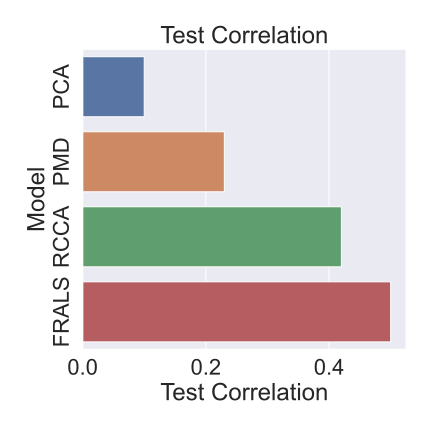
\includegraphics[width=0.32\linewidth]{figures/als/barcorr}
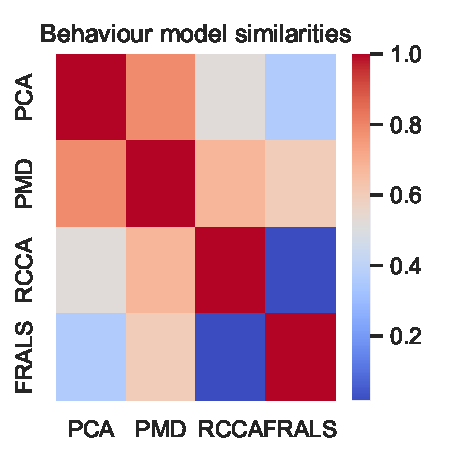
\includegraphics[width=0.32\linewidth]{figures/als/behaviour_model_similarities}
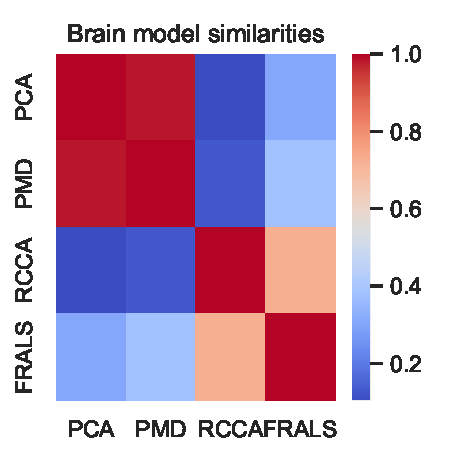
\includegraphics[width=0.32\linewidth]{figures/als/brain_model_similarities}
\caption{Left: Out-of-sample canonical correlations for each model. Middle: Correlation matrix of the scores for each modality. Right: Correlation matrix of the brain loadings for each model.}
\label{fig:performance}
\end{figure}

\subsubsection{Behaviour and Brain Loadings}
In terms of behavioral loadings, except for PCA, all models identified a latent variable that correlated positively with cognitive tests and negatively with cigarette, tobacco, or alcohol use.
Both RCCA and FRALS demonstrated stronger correlations with the Line Orientation test, which measures visuospatial abilities.

\begin{figure}[h]
\centering
\includesvg[width=\linewidth]{figures/all_top_and_bottom_loadings.svg}
\label{fig:behaviour}
\caption*{Top 5 positive and negative non-imaging loadings for each model}
\end{figure}

Regarding the brain loadings, our analysis shows that each model assigns different weights to various brain regions
based on their connectivity.
RCCA and FRALS assigned more weight to the parietal lobe, known for its role in visuospatial processing, than did PCA and PMD. This suggests that the parietal lobe is more relevant for the brain-behaviour correlations captured by our model.
Conversely, PMD appears to rely on principal components in the brain, potentially missing the true associations between the views.
FRALS functions as a sparse version of RCCA in this context.

\begin{figure}[h]
\centering
\includegraphics[width=0.49\linewidth]{figures/als/pca_brain_loadings.pdf}
\includegraphics[width=0.49\linewidth]{figures/als/pmd_brain_loadings.pdf}
\includegraphics[width=0.49\linewidth]{figures/als/rcca_brain_loadings.pdf}
\includegraphics[width=0.49\linewidth]{figures/als/flexals_brain_loadings.pdf}
\caption*{Map of CCA connection strength increases/decreases, with each node’s parcel map weighted by CCA edge-strength increases, summed across edges involving that node.}
\label{fig:brain}
\end{figure}

\section{Discussion}


\section{Limitations}\label{sec:limitations}

While FRALS offers promising performance in terms of out-of-sample correlation, it does come with significant drawbacks, the most noteworthy being its computational inefficiency. Below, we outline the primary factors contributing to the slow speed of FRALS and provide some insights into the computational bottlenecks.

\subsection{Computational Time}\label{subsec:computational-time}
One of the major constraints of FRALS is the time complexity involved in solving the regularized least squares regressions to completion. The algorithm’s iterative nature, which involves solving a sequence of regressions, makes it computationally intensive, particularly when dealing with high-dimensional data.

\begin{figure}[h]
\centering
\includegraphics[width=0.6\linewidth]{figures/time_comparison.png}
\caption{Time comparison between FRALS and other CCA methods}
\end{figure}

\subsection{Changing Regression Targets}\label{subsec:changing-regression-targets}
Adding to the computational burden is the fact that the regression targets, i.e., the projections of the other view, are not static but change dynamically throughout the algorithm's run.
Each update to the least squares solution consequently alters the global objective, leading to a constantly shifting landscape that the algorithm needs to navigate.





\subsection{Conclusions and Further Work}
The main idea of this chapter is to introduce FRALS, a novel approach in the realm of multiview learning that optimizes
both flexibility and performance.
Our experiments indicate that FRALS not only outperforms established methods like PCA, PMD, and RCCA in terms of out-of-sample canonical correlations but also captures novel and distinct aspects of brain-behavior associations.
This uniqueness is evident from the low or negative correlations FRALS holds with other models.

Our findings also underline the importance of the parietal lobe in understanding brain-behavior associations.
FRALS emphasizes this region more compared to traditional methods like PCA and PMD. Future work should focus on understanding the specific functions and contributions of different brain regions captured by FRALS and how they relate to various behaviors.

Given its promising initial results, the next step for FRALS would be its application to larger datasets and its adaptation for different kinds of biological and non-biological data to further evaluate its robustness and applicability.



\section{Conclusion}

We have introduced a flexible and efficient framework for regularized CCA that addresses the limitations of existing methods.
Our framework is particularly well-suited for high-dimensional data and can be adapted to various types of regularization, offering an effective tool for uncovering complex relationships in multiview data.









% \chapter{Gradient Descent: Accelerating CCA for Large Datasets}\label{ch:gradient_descent}
The content of this chapter is based on a preprint paper where I am first author.
I initiated the project based on heuristic arguments and contacted coauthors Ana Lawry Aguila (who provided and analysed the UK Biobank data) and Lennie Wells (who provided extensive mathematical proofs which are in the appendix of this PhD thesis for the interest of the reader).
Both of my coauthors helped me to revise the manuscript.
\minitoc

\section{Introduction}

Subspace learning techniques such as Canonical Correlation Analysis (CCA) have been essential tools in various scientific domains.
While these techniques are powerful, they face computational and scalability challenges, particularly for large datasets.
The focus of this chapter is to explore methods to effectively implement CCA using gradient descent and further scale it using stochastic gradient descent.
This chapter serves as a foundation for the application of proximal gradient descent in regularisation, which will be discussed in subsequent chapters.

\subsection{Problem Statement}

The existing methodologies for solving Canonical Correlation Analysis (CCA) face severe computational limitations, especially for large-scale datasets.
The challenges include high computational intensity and memory demands.

\subsection{Contributions}

This chapter introduces a principled framework for subspace learning and Self-Supervised Learning (SSL) aimed at accelerating and scaling CCA. The contributions are:

\begin{itemize}
  \item Proposing an effective approach to solve CCA using gradient descent, laying the groundwork for future regularisation techniques using proximal gradient descent.
  \item Introducing a scalable methodology for applying CCA to large-scale medical datasets through stochastic gradient descent.
  \item Demonstrating the framework's effectiveness and scalability across diverse tasks and datasets.
  \item Providing a unique real-world application of stochastic PLS on an extremely high-dimensional biomedical dataset.
\end{itemize}

The subsequent sections will elaborate on these contributions, validating our approaches through various experimental setups and real-world applications.


\section{Background}
\subsection{Reconstruction perspective on PCA and CCA}
The key idea behind this chapter relies on treating CCA as a low-rank approximation problem, rather than a constrained optimization problem or a generalized eigenvalue problem.

While this perspective is unusual in the context of CCA, it is well-known in the context of PCA. Indeed, the Eckart-Young-Mirsky theorem \cite{stewart_matrix_1990} states that the best rank-$k$ approximation to a matrix $M$ is given by the truncated SVD:

\begin{align}
    \argmin_{\substack{W \in \R^{d \times k} \\ W^T W = I}} \| M - W W^T M \|_F^2 = U_k \Sigma_k V_k^T
\end{align}

where $U_k \Sigma_k V_k^T$ is the truncated SVD of $M$. If we consider the case where $M=XX^T$, then this is precisely the PCA problem. 

This is a well-known result in matrix analysis, and it is often used to motivate PCA as a low-rank approximation problem. 
This reconstruction perspective is also the basis behind the Autoencoder, a popular deep learning architecture \cite{goodfellow2016deep}, which can be seen as a non-linear generalisation of PCA. 

In this chapter, we will show that a similar result holds for CCA and Generalized Eigenvalue Problems more generally, and that this can be used to motivate a new formulation of CCA as a low-rank approximation problem.

\section{Data}
\subsection{MediaMill}
The MediaMill dataset \cite{feng2004context} is a benchmark dataset for multilabel classification. It consists of 1200 video clips from the TRECVID 2003 conference, each annotated with 101 labels. The original goal of the dataset was to predict the labels of the videos from the visual and audio features. It has since become a benchmark dataset for CCA and other multiview learning methods. We use the same features as \cite{gemp2022generalized} which are 128-dimensional bag-of-visual-words features and 13-dimensional bag-of-audio-words features. We split the data into 80\% train and 20\% test and use cross-validation within the training data in order to tune hyperparameters.

\subsection{Split CIFAR}
The CIFAR-10 dataset \cite{krizhevsky2009learning} consists of 60,000 32x32 colour images in 10 classes, with 6000 images per class. There are 50,000 training images and 10,000 test images. We split the images into two halves.

\subsection{UK Biobank}
The UK Biobank (UKBB) is arguably the largest scale biomedical database in the world with around half a million total participants. The goal is to have imaging data for the brain, heart, and body for 100,000 participants. The UK Biobank combines these images with genetics, biomarkers, electronic health record, and online questionnaires making it a rich dataset for broad studies of health.

For the GEP-EY PLS analysis on biomedical data, we used 33,333 subjects from the UK Biobank \cite{sudlow2015uk}. We used pre-processed (using FreeSurfer \cite{Fischl2012}) grey-matter volumes for 66 cortical (Desikan-Killiany atlas) and 16 subcortical brain regions and 582,565 autosomal genetic variants. The affects of age, age squared, intracranial volume, sex, and the first 20 genetic principal components for population structure were removed from the brain features using linear regression to account for any confounding effects. Each brain ROI was normalised by removing the mean and dividing the standard deviation. We processed the genetics data using PLINK \cite{Purcell2007} keeping genetic variants with a minor allele frequency of at least 1\%  and a maximum missingness rate of 2\%. We used mean imputation to fill in missing values and centered each variant.

To generate measures of genetic disease risk, we calculated polygenic risk scores using PRSice \cite{PRSice2014}. We calculated scores, with a p-value threshold of 0.05, using GWAS summary statistics for the following diseases; Alzheimer's \cite{Lambert2013}, Schizophrenia \cite{Trubetskoy2022}, Bipolar \cite{Mullins2021}, ADHD \cite{Demontis2023}, ALS \cite{Van_Rheenen2021}, Parkinson's \cite{Nalls2019}, and Epilepsy \cite{International_League_Against_Epilepsy_Consortium_on_Complex_Epilepsies2018}, using the referenced GWAS studies.


\section{Methods}

In this section, we introduce a new class of algorithms based on matrix analysis results which allow us to efficiently solve a number of interesting problems including but not limited to CCA, PLS, DCCA, and SSL.

\subsection{GEP-GHA}
First, we present GEP-GH.

\begin{restatable}[Eckhart-Young inspired objective for GEPs]{proprep}{GHAcharac}
    \label{prop:GHA-charac}
    The top-$k$ subspace of the GEP $(A,B)$ can be characterised by maximising the following objective over $W \in \R^{d \times k}$:
    \begin{align}
        \mathcal{U}^\text{GEP-GHA}(W) \defeq \tr \left( 2\, W^T A W - \left(W^T A W\right) \left(W^T B W\right) \right)
    \end{align}
    Moreover, the maximum value is precisely $\sum_{j=1}^k \lambda_j^2$, where $(\lambda_j)$ are the generalised eigenvalues.
\end{restatable}

\subsection{GEP-EY: an unconstrained objective for GEPs}

First, we present GEP-EY, a formulation of GEP problems by matrix analysis which permits efficient optimization by gradient descent.
This is summarised by proposition \ref{prop:EY-charac}, a consequence of applying the Eckhart-Young-Minsky inequality \cite{stewart_matrix_1990} to the eigen-decomposition of $B^\mhalf A B^\mhalf$. Detailed statements and proofs can be found in supplement \ref{supp:proofs}.
%L: of applying EY to the GEP formulation

\begin{restatable}[Eckhart-Young inspired objective for GEPs]{proprep}{EYcharac}
    \label{prop:EY-charac}
    % The top-$k$ subspace of a positive semi-definite GEP $(A,B)$ can be characterised by:
    % \begin{align}\label{eq:EY-charac}
    %     \max_{W \in \R^{d \times k}} \mathcal{U}^\text{GEP-EY}(W) \defeq \tr \left( 2\, W^T A W - \left(W^T B W\right) \left(W^T B W\right) \right).
    % \end{align}
    The top-$k$ subspace of the GEP $(A,B)$ can be characterised by maximising the following objective over $W \in \R^{d \times k}$:
    \begin{align}
        \mathcal{U}^\text{GEP-EY}(W) \defeq \tr \left( 2\, W^T A W - \left(W^T B W\right) \left(W^T B W\right) \right)
    \end{align}
    Moreover, the maximum value is precisely $\sum_{j=1}^k \lambda_j^2$, where $(\lambda_j)$ are the generalised eigenvalues.
\end{restatable}



In the following sections, we describe a number of algorithms for solving GEPs using proposition \ref{prop:EY-charac}.
These will be denoted with \textbf{EY}.

\subsection{Stochastic Optimization}

We next show how GEP-EY and CCA-SVD can be efficiently optimized using stochastic methods, which makes them suitable for large-scale and online settings.
Suppose we have an unbiased estimate $\hat{A}$ for $A$ and a pair of independent and unbiased estimates $(\hat{B},\hat{B}')$ of the matrix $B$ (for example obtained from a minibatch); then one can estimate the objective in proposition \ref{prop:constr-charac} by:
\begin{align}
    \hat{\mathcal{U}}^\text{GEP-EY}(W) \defeq \tr \left( 2\, W^T \hat{A} W - \left(W^T \hat{B} W\right) \left(W^T \hat{B}' W\right) \right)
\end{align}
which we can differentiate to give a gradient estimate:
\begin{align}\label{eq:GEP-EY-grad}
    \hat{\Delta}^{\text{GEP-EY}}(W)
    \defeq \nabla_W \hat{\mathcal{U}}^\text{GEP-EY}(W)
    % old = 4 \left\{ \hat{A} W - \hat{B} W \left(W^T \hat{B}' W \right) \right\}
    = 2 \left\{ 2 \hat{A} W - \hat{B} W \left(W^T \hat{B}' W \right) - \hat{B}' W \left(W^T \hat{B} W \right) \right\}
\end{align}

By the independence of $(\hat{B},\hat{B}')$ both of these estimates are unbiased.

The unbiased estimate immediately leads to Algorithm \ref{alg:Delta}.
The key advantage of this is that the computational complexity of the algorithm is only $\mathcal{O}(b d k)$; this is far less than the $\mathcal{O}(N d^2)$ complexity of any methods which evaluate the matrices $A,B$ on the full batch.

\textit{Why is the complexity so low?} Because $A,B$ are linear functions of covariance matrices, we can construct our unbiased estimates by plugging in sample covariances on a minibatch.
These estimates will then be low rank; indeed we can factorise these estimates in the form $\hat{M} \hat{M}^T$ where $\hat{M} \in \R^{d \times b}$. The dominant cost in evaluating $\mathcal{U}^\text{GEP-EY}$ is then just the matrix multiplications of the form $\hat{M}^T W$; see supplement \ref{supp:analyticsubspace} for full details.

\begin{algorithm}
    \caption{GEP-EY: A Stochastic Gradient Descent Algorithm for GEP subspace}
    \label{alg:Delta}
    \begin{algorithmic}
        \STATE {\bfseries Input:} data stream $Z_t$ consisting of B samples from $z_n$. Learning rate $(\eta_t)_t$. Number of time steps $T$. Number of eigenvectors to compute $k$.
        \STATE {\bfseries Initialise:} $(\hat{\mathbf {W}})_{i=1}^K$ with random uniform entries
        \FOR{$t=1$ {\bfseries to} $T$}
        \STATE Construct an independent unbiased estimate of $\hat{A}$ and two independent unbiased estimates of $\hat{B}$ from $Z_t$
        \STATE $\hat{\mathbf {W}} \leftarrow \hat{\mathbf {W}}+\eta_{t} \hat{\Delta}^{\text{GEP-EY}}$
        \COMMENT{As defined in (\ref{eq:GEP-EY-grad})}
        \ENDFOR
    \end{algorithmic}
\end{algorithm}

\section{Experiments and Results}

%%%%%%%%%%%%%%%%%%%%%%%%%%%%%%%%%%%%%%%%%%%%%%%%%%%%%%%%%%%%%%%%%%%%%%%%%%%%%%%%%%%%%%
%Stochastic CCA
%%%%%%%%%%%%%%%%%%%%%%%%%%%%%%%%%%%%%%%%%%%%%%%%%%%%%%%%%%%%%%%%%%%%%%%%%%%%%%%%%%%%%%
\subsection{Experiment 1: Application of CCA-EY to stochastic CCA}

In this section, we compare GEP-GD and CCA-SVD to $\gamma$-EigenGame \cite{gemp2022generalized} and SGHA \cite{chen2019constrained} for approximating CCA in the stochastic setting. Replicating the experiment in \cite{meng2021online, gemp2022generalized}, we optimize for the top-4 CCA subspace for the MediaMill and Split CIFAR (left and right halves of CIFAR-10 images) datasets. We use a minibatch size 100 and train for one epoch across 5 random seeds (with 1 standard deviation error bars in the plots). We use the Scipy \cite{virtanen2020scipy} package to solve the full batch GEPs as a ground truth value and use the proportion of correlation captured (PCC) captured by the learnt subspace as compared to this ground truth (defined in supplement \ref{supp:experimental details}). Unlike \cite{gemp2022generalized}, we do not perform PCA on the data before applying the CCA methods but instead, for the MNIST data, we add gaussian noise to avoid zero variance subspaces in $X$ and $Y$. This makes our task more challenging, as performing PCA simplifies the problem by substituting $B$ for the identity matrix $I$. This explains the decrease in performance of $\gamma$-EigenGame as compared to their original work.

Figure \ref{fig:ccaiter} shows that both of our methods outperform SGHA and $\gamma$-EigenGame on both datasets in terms of speed of convergence and achieve near-optimal performance in terms of PCC after just one epoch. All of the algorithms share the same complexity per iteration so that these results are also representative in terms of runtime. This demonstrates the effectiveness and superiority of our method for solving CCA in the stochastic setting.

\begin{figure}%[H]
    \centering
    \begin{subfigure}[b]{0.49\textwidth}
        \centering
        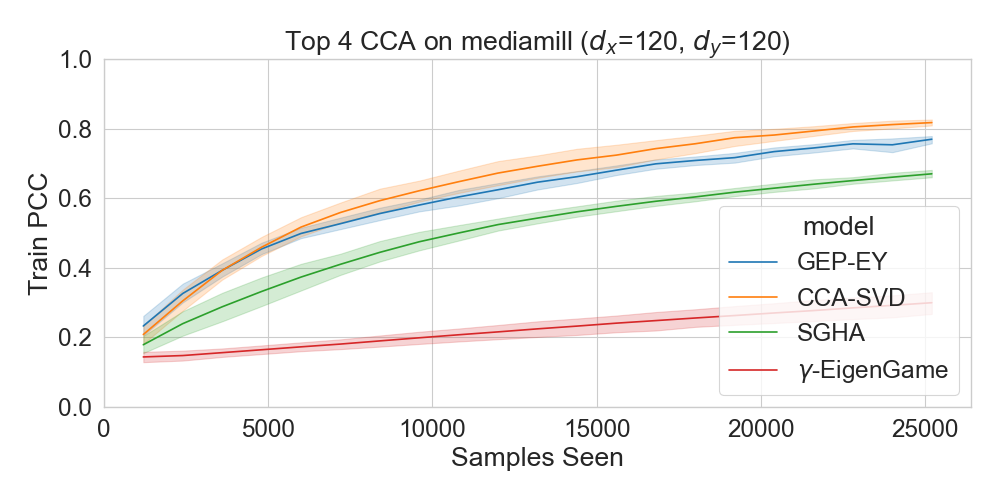
\includegraphics[width=\textwidth]{figures/gradient_descent/CCA/mediamill_100_pcc_lr_tuned.png}
        \label{fig:ccamediamill}
    \end{subfigure}
    \hfill
    \begin{subfigure}[b]{0.49\textwidth}
        \centering
        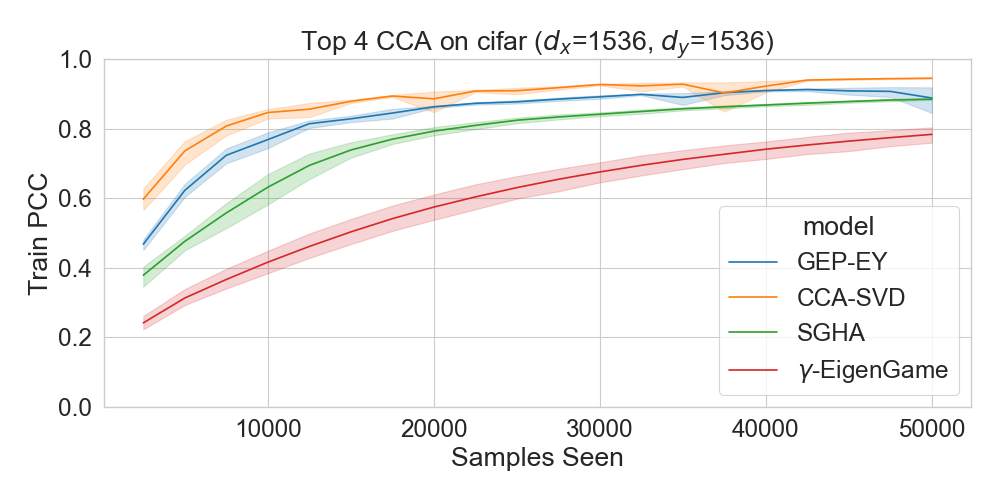
\includegraphics[width=\textwidth]{figures/gradient_descent/CCA/cifar_100_pcc_lr_tuned.png}
        \label{fig:ccacifar}
    \end{subfigure}
    \caption{PCC with respect to Scipy ground truth by GEP-EY and CCA-SVD vs prior work for (a) MediaMill and (b) Split CIFAR data. The maximum value is 1.0 and shading represents $\pm$ 1 standard deviation.}
    \label{fig:ccaiter}
    \label{fig: stochasticcca}
\end{figure}

\subsection{Stochastic CCA Minibatch Size}

\subsection{Exploration of Stochastic CCA Minibatch Size}

\subsection{Stochastic CCA Minibatch Size Examination}

In this section, we take a closer look at how minibatch sizes impact the performance of our method in the stochastic CCA setting. We maintain a constraint of single epoch training. This means that when we use smaller minibatches, the number of training steps increases correspondingly.

Our experiments, as displayed in Figure \ref{fig:minibatch size ablation}, show that our method performs well across a range of minibatch sizes. Notably, it achieves high performance even when the minibatch size is nearly equivalent to the number of components.

This indicates that our method can learn effectively from a limited number of samples. It suggests the possibility of applying our method to analyse large datasets on devices with restricted memory, by processing small minibatches of data sequentially. This robustness to minibatch size could potentially make our method a viable solution for large-scale data analysis where computational resources are limited.

\begin{figure}[h]
    \centering
    \begin{subfigure}[b]{0.49\textwidth}
        \centering
        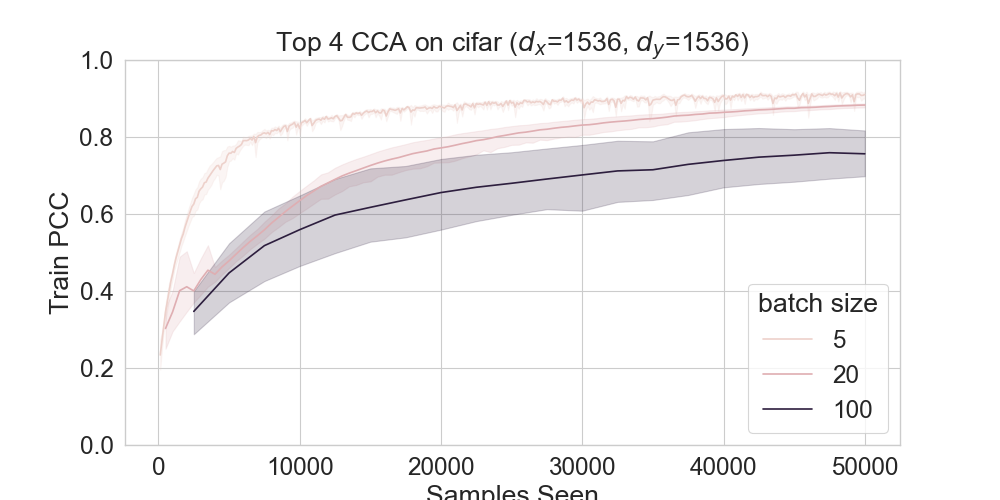
\includegraphics[width=\textwidth]{figures/gradient_descent/CCA/cifar_minibatch_size_ablation.png}
        \caption{}
        \label{fig:cifar_minibatch_ablation}
    \end{subfigure}
    \begin{subfigure}[b]{0.49\textwidth}
        \centering
        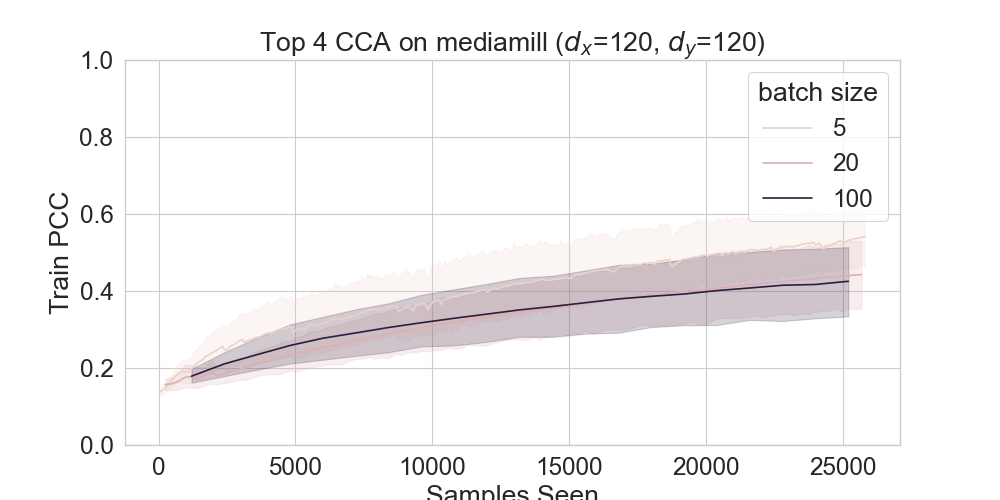
\includegraphics[width=\textwidth]{figures/gradient_descent/CCA/mediamill_minibatch_size_ablation.png}
        \caption{}
        \label{fig:mediamill_minibatch_ablation}
    \end{subfigure}
    \caption{Ablation study on minibatch size for stochastic CCA for (a) cifar and (b) mediamill datasets for minibatch sizes 100, 20, and 5}
    \label{fig:minibatch size ablation}
\end{figure}



%Stochastic PLS UKBB
%%%%%%%%%%%%%%%%%%%%%%%%%%%%%%%%%%%%%%%%%%%%%%%%%%%%%%%%%%%%%%%%%%%%%%%%%%%%%%%%%%%%%%
\subsection{Experiment 2: Application of PLS-EY to PLS on large scale biomedical data}

We demonstrate the power of GEP-EY for large-scale subspace learning by solving PLS on imaging genetics data from the UK Biobank \cite{sudlow2015uk}, a biomedical database. This can reveal novel phenotypes of interest and uncover genetic mechanisms of disease and brain morphometry. Previous imaging genetics analyses using PLS and CCA were limited to small-scale datasets \cite{Lorenzi2018,Taquet2021,Lefloch2012}, which are prone to overfitting and instability. Full batch approaches are infeasible for this data due to the high computational cost. The only other large-scale PLS analysis on the UK Biobank used a federated approach with local batch PLS-SVD \cite{lorenzi2016}, which approximates the global solution. We present the first stochastic PLS analysis on large-scale biomedical data.

We ran GEP-EY with minibatch size 500 on brain imaging (82 regional volumes) and genetics (582,565 variants) data for 33,333 subjects; a massive amount of data that challenges existing methods. See supplement (Section \ref{sec:ukbb_preprocessing}) for data pre-processing details. We see strong validation correlation between all 10 corresponding pairs of vectors in the PLS subspace and weak cross correlation, indicating that our model learnt a coherent and orthogonal subspace of covariation (Figure \ref{fig:UKBB_corr}), a remarkable feat for such high-dimensional data. We found that the PLS brain subspace was associated with genetic risk measures for several disorders (Figure \ref{fig:genetic_risk}), suggesting that the PLS subspace encodes relevant information for genetic disease risk, a significant finding for biomedical research.


\begin{figure}
    \centering
    \begin{subfigure}[b]{0.27\textwidth}
        \centering
        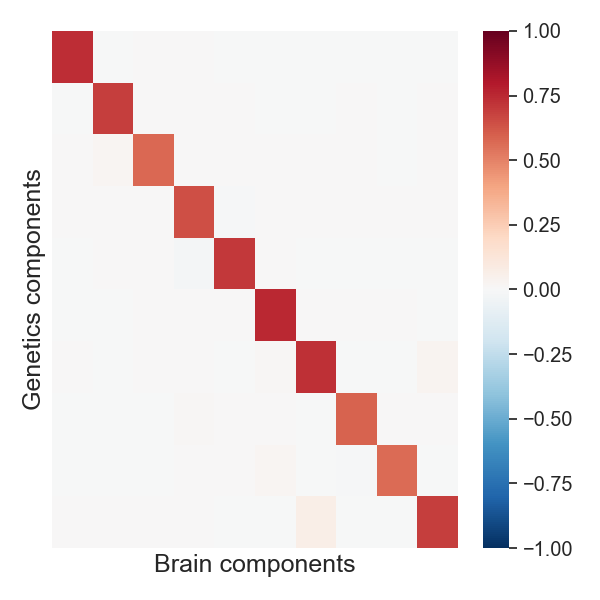
\includegraphics[width=\textwidth,trim={0.8cm 0cm 0.3cm 0cm}]{figures/gradient_descent/UKBB/cross_corr.png}
        \caption{}
        \label{fig:UKBB_corr}
    \end{subfigure}
    \begin{subfigure}[b]{0.72\textwidth}
        \centering
        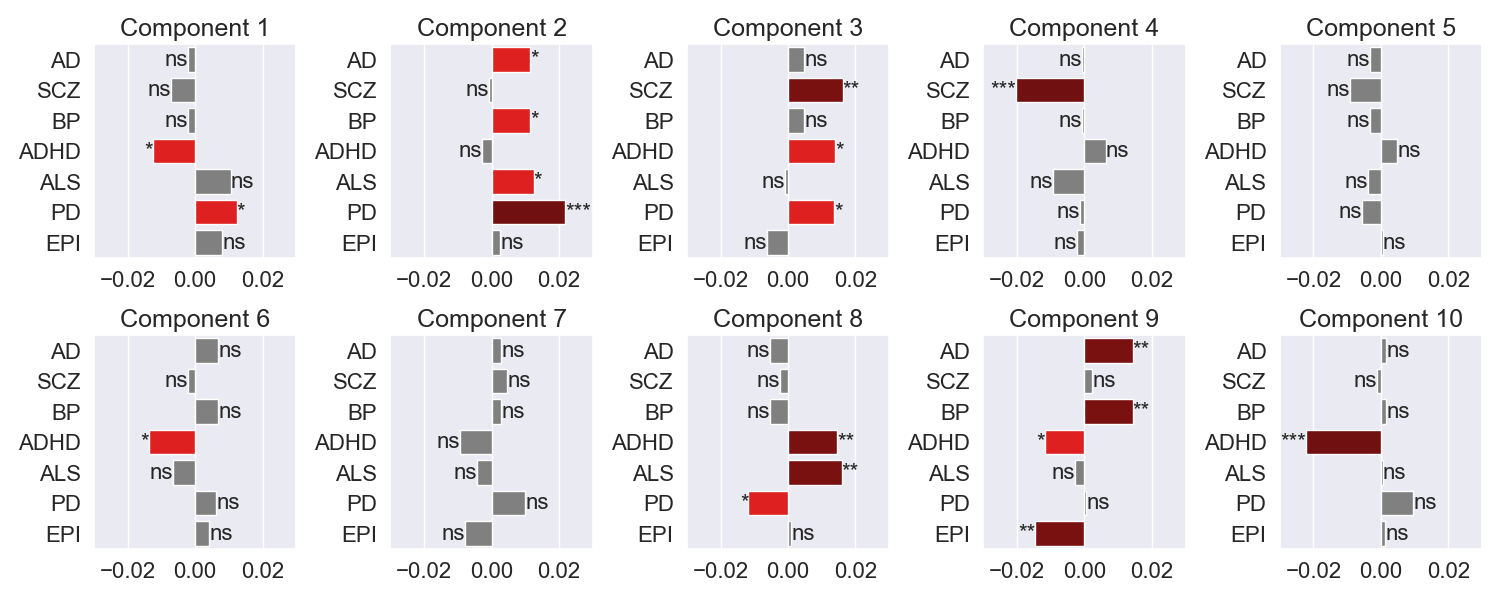
\includegraphics[width=\textwidth,trim={0.5cm 0cm 0.7cm 0cm}]{figures/gradient_descent/UKBB/prs_correlations.png}
        \caption{}
        \label{fig:genetic_risk}
    \end{subfigure}
    \caption{(a) Correlations between PLS components for UK Biobank. (b) Correlations between PLS brain components and genetic risk scores. AD=Alzheimer's disease, SCZ=Schizophrenia, BP=Bipolar, ADHD=Attention deficit hyperactivity disorder, ALS=Amyotrophic lateral sclerosis, PD=Parkinson's disease, EPI=Epilepsy. $\text{ns}: 0.05< p <= 1, \ast: 0.01< p <=0.05, \ast\ast: 0.001< p <= 0.01, \ast\ast\ast: 0.0001< p <= 0.001$.}
\end{figure}

\section{Discussion and Conclusion}

We presented a new unconstrained objective to characterise GEPs; this immediately gave efficient algorithms to solve many subspace learning methods in the stochastic setting with SGD.
Crucially, the gradient estimates are unbiased and cheap to compute.
Moreover, the only hyperparameter is the choice of optimiser.
We will later show how this work can be adapted and applied to optimise regularised GEPs and, in particular, CCA.

% \chapter{Flexible, Scalable Regularization for Generalized Eigenvalue Problems for Multiview Subspace Learning}
\label{Regularised}

The content relating to regularised alternating least squares as a method for optimizing regularised CCA is based on an abstract which I presented in poster form at OHBM. The work benefitted from extensive theoretical discussions with John Shawe-Taylor and Janaina Mourao-Miranda as well as Janaina and Rick Adams' help interpreting the results.

\section{Introduction}

\section{Data}
\subsection{Human Connectome Project (HCP)}

The Human Connectome Project (https://www.humanconnectome.org/study/hcp-young-adult/data-releases) contains structural and resting-state fMRI data as well as behavioural, demographic, and lifestyle measures for 1,200 subjects including 1003 health subjects and a number with mental health conditions such as depression. The original goal of the HCP dataset was to understand the relationships between functional and structural images of the brain. We hypothesize that multiview machine learning will illuminate variations in depression and how it is manifested in the brain by uncovering associations between brain connectivity and non-imaging features (e.g., demographics, psychometrics and other behavioural features)

\subsection{Alzheimer's Disease Neuroimaging Initiative (ADNI)}

The Alzheimer's Disease Neuroimaging Initiative (ADNI) (https://adni.loni.usc.edu/) contains 3 cohorts of subjects with significant overlap. Subjects are labelled as Alzheimer's disease patients, Mild Cognitive Impairment subjects, and elderly controls. The ADNI dataset contains MRI and PET images as well as genetics and cognitive tests. It is aimed at determining the relationships between different biomarkers of Alzheimer's disease and, owing to the strength of the disease signal, has been a benchmark dataset for machine learning and deep learning since its release in 2017. We hypothesize that there are associations between regions of the brain which are damaged by the disease and specific behavioural outcomes like memory.


\section{Contributions}

\subsection{Simulated Data for Comparing Sparse CCA Models}

A necessary 

\subsection{Flexible Regularised ALS}

We can solve CCA by alternating minimisation over each view, based on the alternating least squares form. This form finds a variable $\bold{T}$ that is close to the latent variables $\bold{X}_i\bold{W}_i$, where $\bold{X}_i$, $\bold{W}_i$ are the matrix and weights for each view $i$. The closer $\bold{T}$ is to $\bold{X}_i\bold{W}_i$, the higher the correlation between them. The constraint  $\bold{T^{\top}T}=\bold{I}$ ensures that the latent space is orthogonal to find different effects.

\[ \underset{\bold{W},\bold{T}}{\mathrm{argmin}}\left\{\sum_i \|\bold{X}_i\bold{W}_i-\bold{T}\|_{F}^2 \right\} \]
  \[ \text{subject to: } \bold{T^{\top}T}=\bold{I} \]

To regularise the projection matrices, we add penalty terms to the objective function, such as $P(\bold{W}_i)=\lambda_i\|\bold{W}_i\|_F$ for ridge regression or $P(\bold{W}_i)=\lambda_i\|\bold{W}_i\|_1$ for lasso. This can help us avoid overfitting and improve the interpretability of the results. This means that \textbf{any regularised least squares solver} can be used to solve each subproblem, such as ridge regression, lasso, elastic net, etc. making our framework substantially more flexible than prior work.

\[ \underset{\bold{W},\bold{T}}{\mathrm{argmin}}\left\{\sum_i \|\bold{X}_i\bold{W}_i-\bold{T}\|_{F}^2 + \textcolor{red}{\lambda_i P(\bold{W}_i)}\}\right\} \]
  \[ \text{subject to: } \bold{T^{\top}T}=\bold{I} \]

A benefit of this approach is that neuroimaging practitioners may have existing code for implementing specific regularisation methods in a regression context which can be reused. Furthermore, they may have large dimensions both in features and increasingly in number of samples which benefit from using highly optimised software. 

\subsection{Flexible Regularised GEPs by Proximal Gradient Descent}

\section{Experiments: Flexible Regularised ALS for Brain-Behaviour Associations in the Human Connectome Project}

\subsection{Experiment Design}

Using FRALS, we solve a CCA problem using alternating elastic net regressions with tuned l1 and l2 regularization. We compare our proposed framework to prior work including ridge Regularised CCA (RCCA), Penalized Matrix Decomposition (PMD), commonly referred to in the literature as Sparse CCA but which strictly optimises covariance rather than correlation, and separate Principal Components Analysis (PCA) of the brain and behavioural data. We show that our method improves on RCCA by finding sparse solutions and improves on PMD by optimising a correlation rather than covariance based objective.

We used resting-state fMRI and non-imaging subject measures of 1003 healthy subjects from the 1200-subject data release of the Human Connectome Project (HCP). Following the main steps from \cite{smith2015positive}, we processed the rs-fMRI data into brain connectivity matrices. Like \cite{smith2015positive} we used 145 items of the non-imaging subject measures and removed the same confounding variables. We split the data into 80\% train and 20\% test and used cross-validation within the training data in order to tune hyperparameters.

\subsection{Results}

\subsubsection{Out of sample generalization}

\subsubsection{Model Similarities}

\subsubsection{Brain Loadings}

\subsubsection{Behaviour Loadings}

\section{Experiments: Total Variation Regularisation using Simulated Data}
\subsection{Experiment Design}
\subsection{Results}


\section{Experiments: Total Variation Regularisation of Brain-Behaviour Assocations in the ADNI Data}
\subsection{Experiment Design}
\subsection{Results}

\section{Comparison of Sparse CCA Methods in Simulated Data}
\subsection{Experiment Design}
\subsection{Results}


\section{Discussion and Conclusion}




% \chapter{Extending our work to Deep CCA and Self-Supervised Learning: A Powerful Approach to Multiview Nonlinear Association Learning}

\section{Introduction}
In this chapter, we extend our work to the deep learning setting. We show that our approach can be applied to deep canonical correlation analysis (DCCA) and self-supervised learning (SSL) more generally. We show that our approach is competitive with existing methods on standard benchmarks and that it is much more stable and scalable. We also show that our approach is much more interpretable than existing methods. We conclude that our approach is a powerful new tool for multiview nonlinear association learning.

\section{Background}
\subsection{Deep Learning}
Deep learning has revolutionised machine learning in the last decade. It has led to breakthroughs in many areas including computer vision \cite{krizhevsky2012imagenet}, natural language processing \cite{devlin2018bert}, and reinforcement learning \cite{mnih2015human}. Deep learning has also been applied to many biomedical problems including drug discovery \cite{gawehn2016deep}, medical imaging \cite{litjens2017survey}, and electronic health records \cite{rajkomar2018scalable}.

\subsection{Deep Canonical Correlation Analysis}


\section{Data}

\subsection{Split MNIST}
The Split MNIST dataset \cite{wang2015stochastic} is a standard benchmark for DCCA. It consists of 60,000 images of handwritten digits from the MNIST dataset \cite{lecun1998gradient}. Each image is 28$\times$28 pixels with 1 channel but we split the image into two halves, each of size 28$\times$14 pixels. We use the standard train/test split.

\subsection{XRMB}
The X-Ray Microbeam (XRMB) dataset \cite{westbury1994x} is a multimodal dataset of speech recordings from 139 speakers with acoustic and articulatory features. The acoustic features are 39-dimensional Mel-frequency cepstral coefficients (MFCCs) extracted from the speech recordings. The articulatory features are 12-dimensional vectors of the vertical positions of the tongue, lips, and jaw. The dataset contains 1,429,236 frames of data, with 10,302 frames per speaker. We use the standard train/test split.

\subsection{CIFAR-10 and CIFAR-100}
The CIFAR-10 and CIFAR-100 datasets contain 60,000 images each, with 10 and 100 classes respectively. Each image is 32$\times$32 pixels with 3 channels. We use the standard train/test split.


\section{Methods}

\subsection{DCCA-EY and DCCA-SVD: Extension to Deep CCA}\label{sec:deep-cca}
The GEP-EY and CCA-SVD formulations also lead naturally to new formulations of Deep CCA which solve a more flexible CCA problem but unlike prior work can be optimized efficiently in the stochastic setting. We will refer to these as DCCA-EY and DCCA-SVD.

%L; just moved this up
We derive the DCCA-EY formulation by applying the GEP formulation of CCA (\ref{eq:cca-GEV}) to our DCCA definition. The analogous derivation for DCCA-SVD is left to supplement \ref{supp:algorithm-details}. 

Population DCCA \cite{andrew2013deep} can be defined analogously to population CCA (see section \ref{sec:CCA Definition}):
given input random vectors $X \in \R^{D_x}, Y \in \R^{D_y}$, find neural networks $f,g$ maximising:
\begin{align}\label{eq:DCCA-Andrew}
    \max_{f,g}  \norm{\CCA_K\left(f(X),g(Y)\right)}_2
\end{align}

The GEP formulation becomes:
\begin{equation*}
    A_{fg} = \begin{pmatrix} 0 &\Cov(f(X),g(Y)) \\ \Cov(g(Y),f(X)) & 0 \end{pmatrix}, \qquad
	B_{fg} = \begin{pmatrix}\Var(f(X)) & 0 \\ 0 & \Var(g(Y)) \end{pmatrix}.
\end{equation*}

Proposition \ref{prop:EY-charac} then allows us to rewrite our objective (\ref{eq:DCCA-Andrew}) as:
\begin{align*}
    \norm{\CCA_k\left(f(X),g(Y)\right)}^2 
    = \sum_{j=1}^k \rho_j^2 
    = \max_{W \in \R^{d \times k}} \tr \left( 2\, W^T A_{fg} W - \left(W^T B_{fg} W\right) \left(W^T B_{fg} W\right) \right).
\end{align*}
Therefore DCCA is equivalent to maximising the right hand side with respect to $f,g$ and $W$. To simplify the objective we follow \cite{wang2015stochastic} and reparametrize to consider the `augmented' neural networks $\bar{f} = U^{\top} f, \bar{g} = V^{\top} g$, where $U\in \R^{d_x \times k}, V\in \R^{d_y \times k}$ are such that $W^{\top} = (U^{\top}, V^{\top})$. This gives our final DCCA objective:

\begin{align}\label{eq:DCCA-EY}
    \mathcal{U}^\text{DCCA-EY}(\bar{f},\bar{g}) = \tr(2 \, A_{\bar{f}\bar{g}} - B_{\bar{f}\bar{g}} B_{\bar{f}\bar{g}})
\end{align}

where we need to define:
\begin{align*}
    A_{\bar{f}\bar{g}}
    &= W^T A_{fg} W 
    = \Cov(\bar{f}(X),\bar{g}(Y)) + \Cov(\bar{g}(Y),\bar{f}(X)) \\
    B_{\bar{f}\bar{g}} 
    &= W^T B_{fg} W 
    = \Cov(\bar{f}(X)) + \Cov(\bar{g}(Y))
\end{align*}


By plugging in sample covariances on a minibatch, we can obtain unbiased estimates of $\mathcal{U}^\text{DCCA-EY}(\bar{f},\bar{g})$.

Therefore, we can apply some variant of SGD to optimize equation \ref{eq:DCCA-EY}.

Note that, as in the earlier DCCA work, though we derived the algorithm by considering $f,g$ with output dimensions $d_x,d_y$, we ultimately end up with networks $\bar{f},\bar{g}$ with the same output dimension $k$; we can view these as giving highly correlated $k$-dimensional embeddings of our data.

\subsection{SSL-EY and SSL-SVD: Application to Self-Supervised Learning}

Finding highly correlated embeddings is a natural objective for SSL.
To apply the previous ideas to joint embedding methods, we simply apply (\ref{eq:DCCA-EY}) in the Siamese pair setting where $\bar{f}=\bar{g}$ are the same map from input data to embeddings (composition of encoder and projector).

We therefore obtain the objective:
\begin{align}\label{eq:SSL-EY}
    \mathcal{U}^\text{SSL-EY}(\bar{f}) =\tr( 2 \, A_{\bar{f}} - B_{\bar{f}} B_{\bar{f}})
\end{align}
where:
\begin{align*}
    A_{\bar{f}}
    &= \Cov(\bar{f}(X),\bar{f}(X')) + \Cov(\bar{f}(X'),\bar{f}(X)) \\
    B_{\bar{f}} 
    &= \Var(\bar{f}(X)) + \Var(\bar{f}(X')).
\end{align*}

Once again, we define SSL-SVD by analogy in supplement \ref{supp:algorithm-details}. We will see in section \ref{Experiments} that SSL-SVD and SSL-EY perform similarly in experiments but we show in supplement \ref{supp:previous work} that the SSL-SVD formulation looks closer to existing SSL methods.

\textbf{Implementation Details:} Typical architectures for the encoder and the projector vary depending on the domain and the dataset \cite{balestriero2023cookbook}. For example, for image classification tasks on CIFAR-10 or ImageNet, a common choice for the encoder is a ResNet, while for the projector a linear layer or a two-layer MLP is often used. Common augmentations for images are cropping, flipping, rotating, color jittering, etc. In this work, we adopt standard architectures and augmentations from the literature.


\section{Experiments and Results}

%%%%%%%%%%%%%%%%%%%%%%%%%%%%%%%%%%%%%%%%%%%%%%%%%%%%%%%%%%%%%%%%%%%%%%%%%%%%%%%%%%%%%%
%DCCA Benchmarking
%%%%%%%%%%%%%%%%%%%%%%%%%%%%%%%%%%%%%%%%%%%%%%%%%%%%%%%%%%%%%%%%%%%%%%%%%%%%%%%%%%%%%%
\subsection{Application of DCCA-EY and DCCA-SVD to to Deep multiview learning on toy data}

We now turn to compare our proposed DCCA-EY and DCCA-SVD methods with existing methods for deep canonical correlation analysis (DCCA). We replicate an experiment from \cite{wang2015stochastic} using the left and right halves of MNIST \cite{lecun1998gradient} digits ($n$=60,000) and X-Ray Microbeam (XRMB, $n$=1,429,236) data \cite{westbury1994x}. XRMB is a multimodal dataset of speech recordings from 139 speakers with acoustic and articulatory features. We use minibatch sizes of 100 for 20 epochs, the architectures described in \cite{wang2015stochastic}, and an output dimensionality of 50.  We use the total correlation captured (TCC) of the learnt subspace on the validation set as a metric (defined in supplement \ref{supp:experimental details}).

\begin{figure}
     \centering
     \begin{subfigure}[b]{0.49\textwidth}
         \centering
         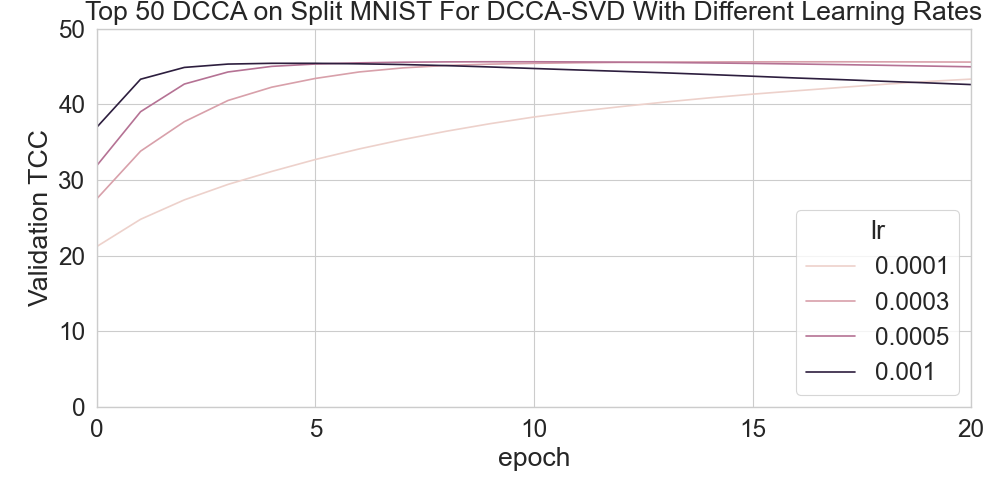
\includegraphics[width=\textwidth]{figures/deep_learning/DCCA/dcca_lr_experiment.png}
         \caption{}
         \label{fig:lrexp}
     \end{subfigure}
     \hfill
     \begin{subfigure}[b]{0.49\textwidth}
         \centering
         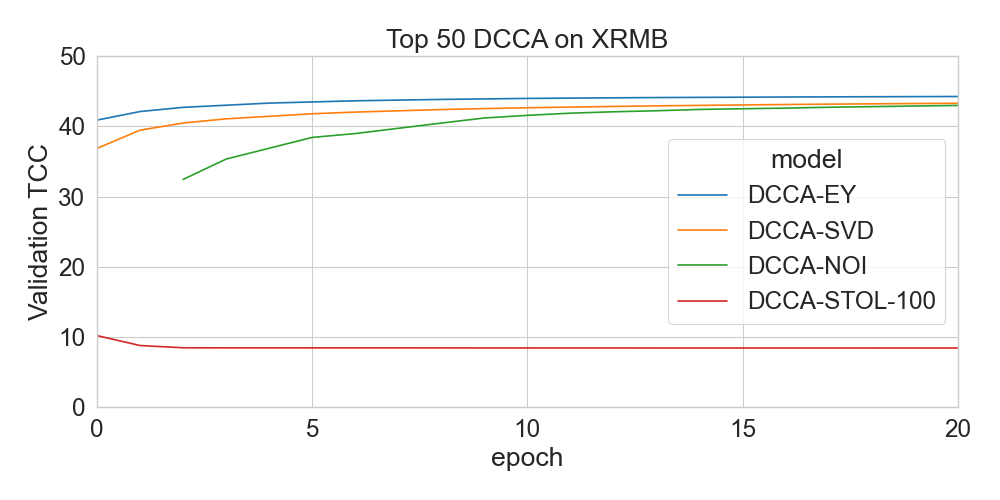
\includegraphics[width=\textwidth]{figures/deep_learning/DCCA/dcca_XRMB.png}
         \caption{}
                 \label{fig:xrmb}
     \end{subfigure}
        \caption{ (a) Validation TCC for different learning rates on Split MNIST data (b) Validation TCC for different methods on XRMB data}

\end{figure}

On the split MNIST data, we show in figure \ref{fig:lrexp} the substantial effect of changing the learning rate on the convergence of the TCC objective. This demonstrates the important of spending computational resource on optimizing the learning rate. An important benefit of our approach is that because the only hyperparameter is learning rate, we can spend all of our computational budget on this critical area. In figure \ref{fig:xrmb}, we show that our proposed methods exhibit extremely fast convergence compared to prior work. Furthermore, both proposed methods find higher validation correlations than DCCA-STOL, showing that they are much more effective ways of estimating the full batch DCCA objective. Note that, the decrease in validation correlation in later epochs is due to overfitting which should be addressed in practical settings by using early stopping as is standard in deep learning.

%%%%%%%%%%%%%%%%%%%%%%%%%%%%%%%%%%%%%%%%%%%%%%%%%%%%%%%%%%%%%%%%%%%%%%%%%%%%%%%%%%%%%%
%SSL
%%%%%%%%%%%%%%%%%%%%%%%%%%%%%%%%%%%%%%%%%%%%%%%%%%%%%%%%%%%%%%%%%%%%%%%%%%%%%%%%%%%%%%
\subsection{Application of SSL-EY and SSL-SVD to Self-Supervised Learning}

In this section, we test our SSL objectives on the CIFAR-10 and CIFAR-100 datasets, which both have 60,000 images and 10 and 100 classes respectively. We compare our methods, SSL-EY and SSL-SVD, with two state-of-the-art methods, Barlow Twins and VICReg. We report k-Nearest Neighbor accuracy on the representations of the validation data in a zero-shot setup.

Firstly, we consider a standard experiment from the literature.
We use the sololearn package \cite{da2022solo}, which includes optimised hyperparameters (and augmentations) for VICReg and Barlow Twins on this specific task.
Each method uses a ResNet-18 encoder, a two-layer projector network with 2048 units in each layer, and is trained for 1,000 epochs with a minibatch size of 256.
For SSL-EY and SSL-SVD, we use the same hyperparameters as Barlow Twins.  
Table \ref{tab:selfsup} shows that our methods are competitive with Barlow Twins and VICReg in this setup.
This is remarkable because their tuning parameters had been heavily optimised, and our method required no tuning at all!

We then performed ablation studies to understand the importance of the (many) hyperparameters in these joint embedding models. In general we found that VICReg was much more sensitive to these hyperparameters than Barlow Twins but that our method was significantly more stable than either of them, see supplement \ref{supp:ablation}.
Table \ref{tab:selfsupsmaller} shows a particularly striking example of this. 
We repeat the previous experiment with all hyperparameters the same apart from the projector: we take a smaller projector with only 256 units in each layer. 
Comparing Tables \ref{tab:selfsup} and \ref{tab:selfsupsmaller} shows that VICReg and Barlow Twins have a large performance drop with the smaller projector on the non-trivial classification problems; our methods are much less affected, and now significantly outperform VICReg and Barlow Twins.
 

\begin{table}[h] 
\centering 
\begin{tabular}{lcccc} 
\hline 
Method & CIFAR-10 Top-1 & CIFAR-10 Top-5 & CIFAR-100 Top-1 & CIFAR-100 Top-5 \\ 
\hline 
Barlow Twins & \textbf{92.1} & 99.73 & \textbf{71.38} & \textbf{92.32}\\
VICReg & 91.68	&99.66 & 68.56&	90.76 \\
\textbf{SSL-EY} & 91.43& \textbf{99.75}& 67.52& 90.17\\
\textbf{SSL-SVD} & 90.57 & 99.71 & 65.93 & 89.31 \\
\hline 
\end{tabular} \caption{SSL methods on CIFAR-10 and CIFAR-100 using 2048 unit projectors.} \label{tab:selfsup}
\centering 
\begin{tabular}{lcccc} 
\hline 
Method & CIFAR-10 Top-1 & CIFAR-10 Top-5 & CIFAR-100 Top-1 & CIFAR-100 Top-5 \\ 
\hline 
Barlow Twins & 88.35 & \textbf{99.71} & 59.94 & 85.99 \\
VICReg & 88.74 & 99.68 & 57.03& 84.45 \\
\textbf{SSL-EY} & 89.49 & 99.54 & \textbf{65.62}& \textbf{89.00}\\
\textbf{SSL-SVD} & \textbf{90.34} & 99.67 & 64.54 & 88.66 \\
\hline 
\end{tabular} \caption{SSL methods on CIFAR-10 and CIFAR-100 using 256 unit projectors.} \label{tab:selfsupsmaller} \end{table}

\section{Discussion and Conclusion}







%\chapter{Identifying Multiview Effects in Subsets of a Population}

\section{Introduction}

Most of the existing methods from multiview machine learning for combining different views of data assume that there is a latent structure common to the whole dataset for example the population lying on a normative spectrum of disease. However the truth may be more complex with some subjects having entirely different sources of variation and possibly even some anomalous subjects. In this chapter, we address the problem of finding multiple associations between views of data when each given sample may contain none, one, or any number of the associations (where we hypothesize that associations between the brain and clinical assessments are driven by or represent mental health variations). In order to tackle this problem, an algorithm must be able to identify both whether a sample contains a given association as well as the nature of the association (i.e. its associated weights). 

One way to formalise this problem is that we would like to build models which have sparsity over subjects or in other words some subjects contribute nothing to the objective in a similar way to how weights sparsity means that some features do not contribute to the objective. When there are two classes with different, but strong associations, classical methods will instead tend to combine the two associations into a shared, weaker association since subject sparsity is not built into the PCA, PLS, or CCA models. This is problematic both for interpreting the association and for separation of different conditions in a mental health context.

Progress on this work has so far been limited to understanding existing approaches to the problem and preliminary research on methods for addressing the problem. 

\section{Related Work}
\label{Related Work}

There have been a handful of approaches to the CCA problem that induce sparsity over samples. The sparse kernel CCA of \cite{chu2013sparse} finds sparse dual vectors in each view in order to improve robustness of the model by regularisation and to improve efficiency of inference at test time. \cite{fern2005correlation} developed a model with a similar philosophy to k-means clustering, with iterative reassignment between clusters and learning cluster parameters based on minimisation of some criterion. Like k-means clustering, this method requires an a priori assumption about the number of clusters and an assumption that there is a correlation between the views for all samples. 

\subsection{A metamorphosis of Canonical Correlation Analysis into Multivariate Maximum Margin Learning}

\cite{szedmak2007metamorphosis} developed a convex optimisation problem which is related to both the CCA problem and the one-class SVM. 

They start with the Rayleigh Quotient form for CCA:

\begin{align}
    & \bold{w_{opt}}=\underset{\bold{w}}{\mathrm{argmax}}\{\frac{ \bold{w_x^{\top}X^{\top}Yw_y } }{\|\bold{Xw_x}\|\|\bold{Yw_y}\|}\}\\
\end{align}

\begin{align}
    \bold{w_{opt}}=\underset{\bold{w}}{\mathrm{argmax}}\{\frac{\left\langle\mathbf{Y}, \mathbf{X} \mathbf{w}_{x} \mathbf{w}_{y}^{T}\right\rangle_{F}}{\|\mathbf{Y}\|_{F}\left\|\mathbf{X} \mathbf{w}_{x} \mathbf{w}_{y}^{T}\right\|_{F}}\}=\underset{\bold{w}}{\mathrm{argmin}}\{\frac{\|\mathbf{Y}\|_{F}\|\mathbf{X} \hat{\mathbf{W}}\|_{F}}{\langle\mathbf{Y}, \mathbf{X} \hat{\mathbf{W}}\rangle_{F}}\}\\
\end{align}

\begin{align}
    \bold{W_{opt}}=\underset{\bold{W}}{\mathrm{argmin}}\{ \|\mathbf{X}\mathbf{W}\|_{F}\} \\
    \text{subject to:} \notag\\ 
    \langle\mathbf{Y}, \mathbf{X} \mathbf{W}\rangle_{F} \geq 1
\end{align}


Before finally proposing a solution with a soft margin. In the case that the data dependence in $\|X_2W\|_F$ is ignored in place of $\|W\|_F$ (an assumption similar to the regularisation effect of PLS with respect to CCA):

\begin{align}
    & \bold{W_{opt}}=\underset{\bold{W}}{\mathrm{argmin}}\{\|\bold{W}\|^2_F + C\bold{1}^{\top}\xi\}\\
    & \text{subject to:} \notag\\
    & \bold{x^{(i)}_2 W x^{(i)}_1}  >=1-\xi_i \notag\\
\end{align}

By considering the slack variables $\xi_i$ as indicators of samples lacking the underlying correlation, this method can be used to select samples which do not share the correlation by considering those with $\xi_i > 0$ as negative samples.

\subsection{Sample Weighted PLS}\label{Sample Weighted PLS}
\cite{wenwen2018sparse} develop what they call a weighted sparse CCA method which learns a sparse sample weight vector as well as the weight vectors for each view which allows them to learn a model of a signal which exists in some samples but not others. This is described by the optimisation problem:

\begin{align}
    & \bold{w_{opt}}=\underset{w}{\mathrm{argmax}}\{ \bold{w_1^{\top}X_1^{\top}\text{diag}(d)X_2w_2  }\}\\
    & \text{subject to:} \notag\\
    & \bold{w_1^{\top}w_1}=1 \notag\\
    & \bold{w_2^{\top}w_2}=1 \notag\\
    & \bold{d^{\top}d}=1 \notag
\end{align}

Which they suggest to solve by alternating optimisation over $\bold{w_1}$ and $\bold{w_2}$. Their algorithm is performant on certain types of data but has a tendency to have large weights (the elements of $\bold{d}$) on a small subset of the samples rather than selecting all of the correlated samples more uniformly. In addition the constraints on $\bold{w_i}$ are PLS constraints rather than CCA constraints implying an assumption of diagonal covariance. For this reason in comparison we will refer to this algorithm as Sparse Weighted PLS. Finally, they show that in principle we can further regularise the weights since it only changes the subproblems in the alternating minimisation.


\subsection{Correlation Clustering}\label{sec:corrclus}

The final algorithm we review here is the correlation clustering algorithm from \cite{fern2005correlation}. The basic steps of the algorithm are somewhat like the expectation maximisation algorithm for k-means clustering. The algorithm alternates between a model fitting step in which $k$ CCA models are fit 

\vspace{\baselineskip}
\begin{algorithm}
\begin{algorithmic}[1]
\STATE {Finds regression model parameters which best fit the data}
\STATE {$k=$ maximum iterations}
\STATE {$n=$ minimum number of samples in each fit, typically the minimum number required by the model e.g. the number of parameters for regression}
\STATE {$t=$ threshold for point to be considered well fit}
\WHILE {iterations $< k$}
    \STATE Randomly assign instances to the $k$ clusters.
    \STATE For $i=1 \cdots k$, apply CCA to cluster $i$ to build $M^{i}=\left\{\left(u_{j}, v_{j}\right), r_{j},\left(a_{j}, b_{j}\right): j=1 \cdots d\right\}$, i.e., the top $d$ pairs of canonical variates, the correlation $r$ between each pair, and the corresponding $d$ pairs of projection vectors.
    \STATE Reassign each instance to a cluster based on its $\vec{x}$ and $\vec{y}$ features and the $k$ CCA models.
    \STATE If no assignment has changed from previous iteration, return the current clusters and CCA models. Otherwise, go to step 2 .
\ENDWHILE
\caption[Correlation Clustering]{Correlation Clustering}
\label{alg:Correlation Clustering}
\end{algorithmic}
\end{algorithm}

\section{Contributions}

\begin{itemize}
    \item \textbf{Contribution 1:} Formulating PCA, PLS and CCA as Maximum Margin Robot formulations and considering how they can be used to select population subsets containing the relevant signal
    \item \textbf{Contribution 2:} An adjusted form of the Weighted PLS from section \ref{Sample Weighted PLS} based on alternating optimisation with better convergence properties
\end{itemize}

\section{\textbf{Contribution 1:} Maximum Margin Robots for Dimensionality Reduction in the Presence of Outliers}

\subsection{Maximum Margin PCA}

Since our interest in the maximum margin formulation of CCA to identify which samples contain the signal of interest, it is interesting to first study the (arguably) simpler problem of PCA to better understand the properties of the Maximum Margin Robot and the types of scenarios where it is most effective. We can write a PCA 

\begin{align}
    & \bold{W_{opt}}=\underset{W}{\mathrm{argmin}}\{\|\bold{W}\|^2_F + C\bold{1}^{\top}\xi\}\\
    & \text{subject to:} \notag\\
    & \bold{x^{(i)} W x^{(i)}}  >=1-\xi_i \notag\\
\end{align}

\subsection{Maximum Margin CCA}

Similarly, we can add back in the data dependence to the Maximum Margin Robot for PLS to give a CCA-like problem.

\begin{align}
    & \bold{W_{opt}}=\underset{W}{\mathrm{argmin}}\{\|\bold{X_1WX_2^{\top}}\|^2_F + C\bold{1}^{\top}\xi\}\\
    & \text{subject to:} \notag\\
    & \bold{x^{(i)}_1 W x^{(i)}_2}  >=1-\xi_i \notag\\
\end{align}

\section{\textbf{Contribution 2:} An Improved Sparse Weighted CCA}

The constraints defined by \cite{wenwen2018sparse} assume the same approximation as the Penalized Matrix Decomposition described earlier. For this reason, their method is better understood as a form of Sparse Weighted PLS. If we substitute these constraints for the true CCA constraints, the problem can still be solved to a local optimum by alternating optimisation:

\begin{align}
    & \bold{w_{opt}}=\underset{\bold{w}}{\mathrm{argmax}}\{ \bold{w_1^{\top}X_1^{\top}\text{diag}(d)X_2w_2}  \}\\
    & \text{subject to:} \notag\\
    & \bold{w_1^{\top}X_1^{\top}X_1w_1}=1 \notag\\
    & \bold{w_2^{\top}X_2^{\top}X_2w_2}=1 \notag\\
    & \bold{d^{\top}d}=1 \notag
\end{align}

However this method inherits the weaknesses of the Sparse Weighted PLS with respect to the vector $\bold{d}$, namely that this constraint has a tendency toward a peaky distribution with a very large weight on a small number of samples. For this reason, we consider the following change to the constraint:

\begin{align}
    & \bold{w_{opt}}=\underset{\bold{w}}{\mathrm{argmax}}\{ \bold{w_1^{\top}X_1^{\top}\text{diag}(d)X_2w_2}  \}\\
    & \text{subject to:} \notag\\
    & \bold{w_1^{\top}X_1^{\top}X_1w_1}=1 \notag\\
    & \bold{w_2^{\top}X_2^{\top}X_2w_2}=1 \notag\\
    & 0\leq d_i \leq 1 \notag
\end{align}

Once again this problem can be solved by alternating optimisation of $w_1$, $w_2$, and $d$. In this case, the elements of $d$ will be either 0 or 1 depending if the projections for a given sample have a positive product or a negative product.

\section{Experimental Results}

Work so far has been an iterative process of understanding the existing methods as well as investigating their performance in different kinds of simulated data.

In all of the experiments we generate a strong `signal of interest' for a population and add a noisy population without an interesting signal. The goal in our constructions is to successfully recover the correct subspace of the interesting population, ideally by simultaneously classifying subjects as interesting or non-interesting. 

Hyperparameters are approximately tuned to the correct region (e.g. ensuring that not all of the slack variables are zero or all slack variables are active) but not optimized. This is because firstly it is not clear what a good optimization criteria would be and secondly it allows us to explore the properties of the algorithms while avoiding cherry picking.

\subsection{PCA}

\subsubsection{Experiment Design}

In the PCA experiments, we generate data by combining two datasets with the same total variance (sum of eigenvalues). The first, interesting, dataset has a much larger first eigenvalue while the second uninteresting dataset has equal eigenvalues. PCA will naturally tend to combine the largest signals in both datasets. We generate 100 interesting samples and 50 uninteresting samples with 10 features.

We show plots of the the data projected onto the first two `principal components' identified by each model in order to demonstrate how well they capture the true subspace. We provide a ground truth by running PCA on only the interesting samples. We show projections for both the training data as well as held out test data.

In addition we show plots of the effective sample weights for each model. Since each model formulates the problem in a slightly different way we highlight that this means:

\begin{itemize}
    \item PCA: the absolute value of the score of each sample or the rows of $Xw$ where $w$ are the weights that form the first principal component. This is motivated by the fact that samples which are projected to near zero contribute very little to the PCA objective.
    \item MMR: Since the model uses slack variables to allow for low variance samples, we obtain `sample weights' by subtracting these slack variables from 1. This means a sample with a zero slack variable has sample weight equal to one. A sample with a maximal slack variable equal to one would have a sample weight of zero.
\end{itemize}

\subsubsection{Results}

The results in figures \ref{fig:pcalatent} and \ref{fig:pcaweights} show that classical PCA is highly effective at suppressing the low variance data, with the uninteresting 'random' samples all clustered around the centre of the PCA subspace while the interesting 'signal' samples form much of the variance. Nonetheless, an interesting property of MMR is that it fairly cleanly assigns 0 slack variables to the vast majority of the interesting samples giving a clean classification. 

\begin{figure}[H] 
    \centering
    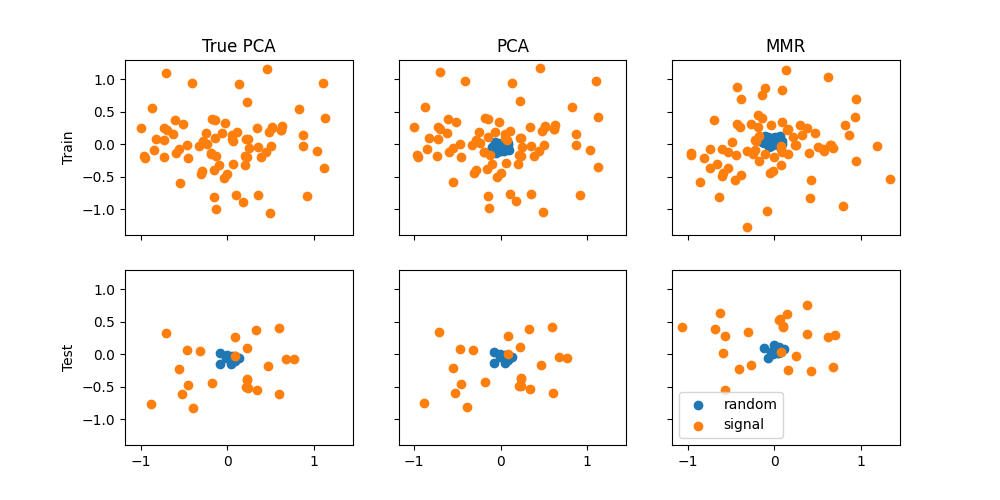
\includegraphics[width=0.9\textwidth]{chapters/sampleselection/pca/models.png}
    \caption{Plots of the first two `principal components' estimated by each model on the x and y axis. The leftmost model is trained using only the interesting data and therefore presents a ground truth}
    \label{fig:pcalatent}
\end{figure}

\begin{figure}[H] 
    \centering
    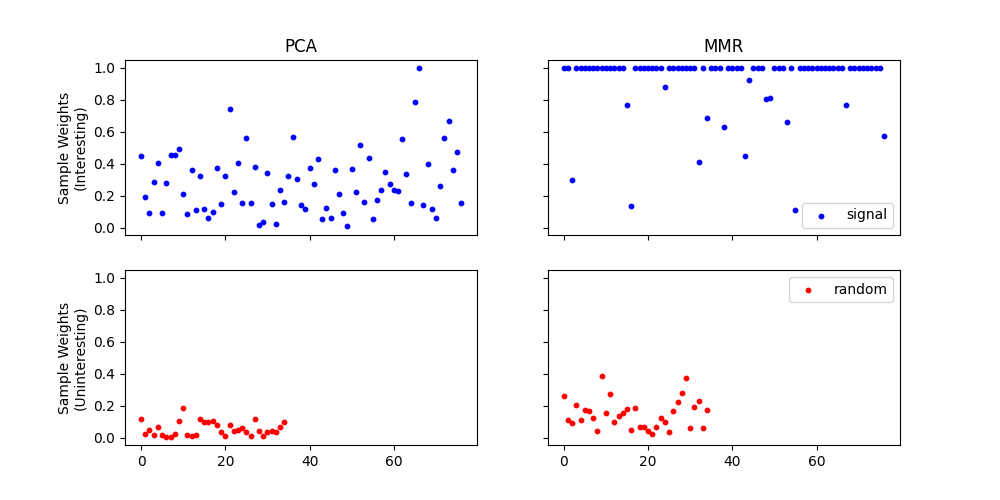
\includegraphics[width=0.9\textwidth]{chapters/sampleselection/pca/weights.png}
    \caption{Plots showing the implied sample weights by both models with the rows separating the interesting samples (top) from the uninteresting samples (bottom). An ideal model would have all samples=1 in the top row and all samples=0 in the bottom.}
    \label{fig:pcaweights}
\end{figure}

\subsection{PLS}

\subsubsection{Experiment Design}

In the PLS experiments, we generate data by combining two multiview datasets. The first is generated using Witten's method described in chapter \ref{chap:framework} while the latter is random noise with the same columnwise variance as the first dataset. We generate 100 interesting samples and 50 uninteresting samples with 10 features in two different views.

One major weakness of using Witten's latent variable model to generate the data with a signal is that the samples associated with the smallest values in the latent variable vector will have lower variance in the data and it is clearly impossible to distinguish between arbitrarily small latent variables and data generated without the latent variables.

We show plots of two views projected onto their first highly covarying latent dimension. We provide a ground truth by running PLS on only the interesting samples. We show projections for both the training data as well as held out test data. The goal for any model is to maximise the covariance of the projections of the `interesting' data.

In addition we show plots of the effective sample weights for each model. Since each model formulates the problem in a slightly different way we highlight that this means:

\begin{itemize}
    \item PLS: The sample wise product of the projections of each view $X_1w_1$ and $X_2w_2$. This is motivated by the fact that samples which drive the covariance objective are those where the projections have the same sign and a large magnitude.
    \item MMR: Since the model uses slack variables to allow for low variance samples, we obtain `sample weights' by subtracting these slack variables from 1. This means a sample with a zero slack variable has sample weight equal to one. A sample with a maximal slack variable equal to one would have a sample weight of zero.
    \item WPLS: The elements of the vector $\bold{d}$ provide a natural sample weighting in their formulation
    
\end{itemize}

\subsubsection{Results}

The results shown in figures \ref{fig:plslatent} and \ref{fig:plsweights} show a degree of promise for using methods which induce sparsity over samples in the PLS context. MMR in particular appears to better suppress the random data when compared to PLS in the latent plots. Interestingly, this is less clear from the sample weighting plots. Our variant of WPLS does not appear to perform well in this context in the sense of successfully recovering the sample weights.

\begin{figure}[H] 
    \centering
    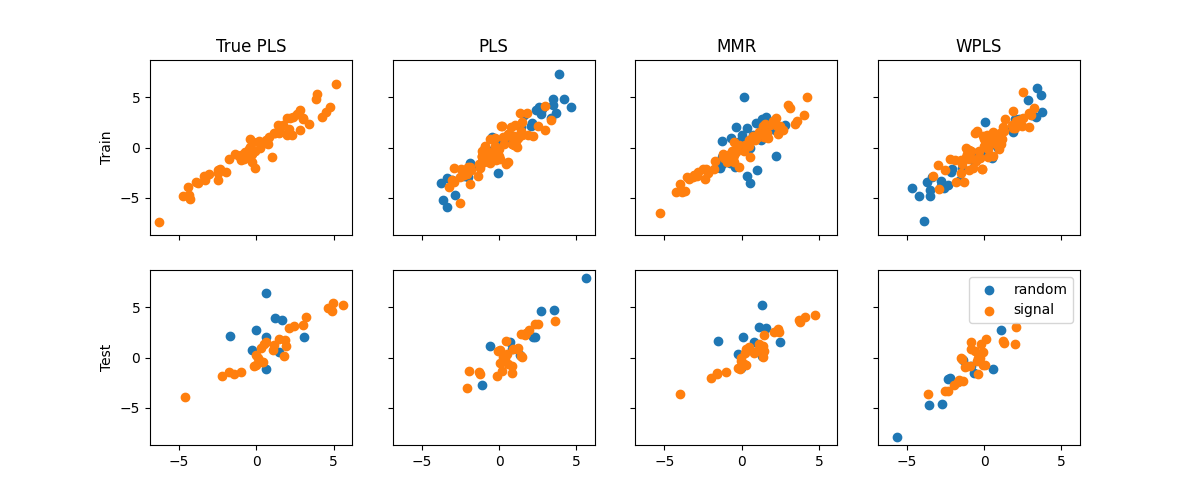
\includegraphics[width=0.9\textwidth]{chapters/sampleselection/pls/models.png}
    \caption{Plots of the first latent score for each view plotted against each other as a scatter plot. The leftmost model is trained using only the interesting data and therefore presents a ground truth}
    \label{fig:plslatent}
\end{figure}

\begin{figure}[H] 
    \centering
    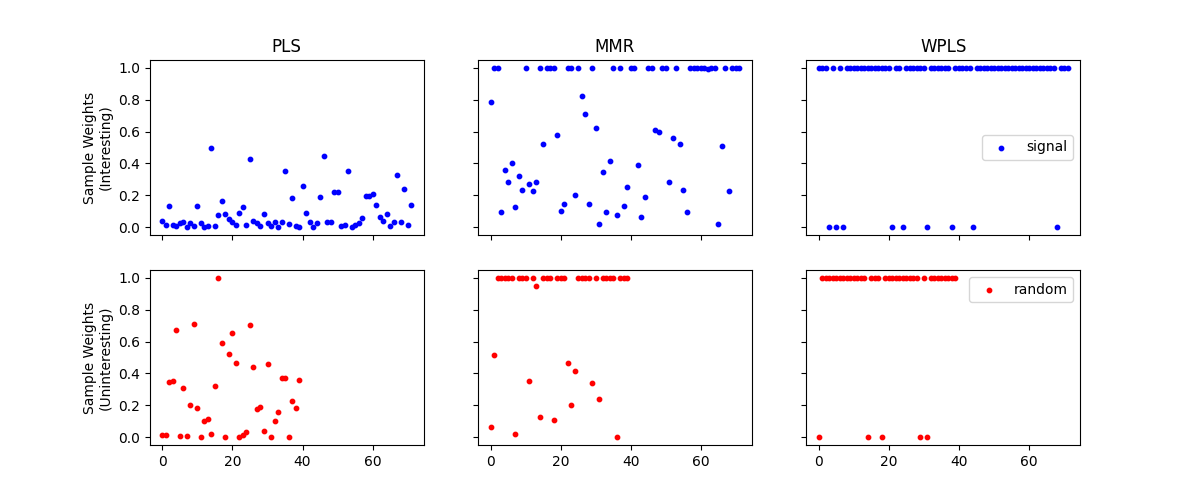
\includegraphics[width=0.9\textwidth]{chapters/sampleselection/pls/weights.png}
    \caption{Plots showing the implied sample weights by both models with the rows separating the interesting samples (top) from the uninteresting samples (bottom). An ideal model would have all samples=1 in the top row and all samples=0 in the bottom.}
    \label{fig:plsweights}
\end{figure}

\subsection{CCA}

\subsubsection{Experiment Design}

In the CCA experiments, data generation follows the same scheme described for the PLS experiments.

We show plots of two views projected onto their first highly correlated latent dimension. We provide a ground truth by running CCA on only the interesting samples. We show projections for both the training data as well as held out test data. The goal for any model is to maximise the correlation of the `interesting data'.

In addition we show plots of the effective sample weights for each model. Since each model formulates the problem in a slightly different way we highlight that this means:

\begin{itemize}
    \item PLS: The sample wise product of the projections of each view $X_1w_1$ and $X_2w_2$. This is motivated by the fact that samples which drive the covariance objective are those where the projections have the same sign and a large magnitude.
    \item MMR: Since the model uses slack variables to allow for low variance samples, we obtain `sample weights' by subtracting these slack variables from 1. This means a sample with a zero slack variable has sample weight equal to one. A sample with a maximal slack variable equal to one would have a sample weight of zero.
    \item WCCA: The elements of the vector $\bold{d}$ provide a natural sample weighting in their formulation
    \item Cluster Correlation: In a binary problem with two groups, we can use the binary classification as a sample weight for visualisation purposes.
\end{itemize}

\subsubsection{Results}

The results shown in figures \ref{fig:ccalatent} and \ref{fig:ccaweights} once again imply some promise for sample selection algorithms. In particular, classical CCA appears to have been driven somewhat by the random data while WCCA and ClusterCorrelation appear to project the interesting samples to a more correlated latent space. The poor performance of MMR suggests a problem with our implementation or construction but is presented for completeness.

\begin{figure}[H] 
    \centering
    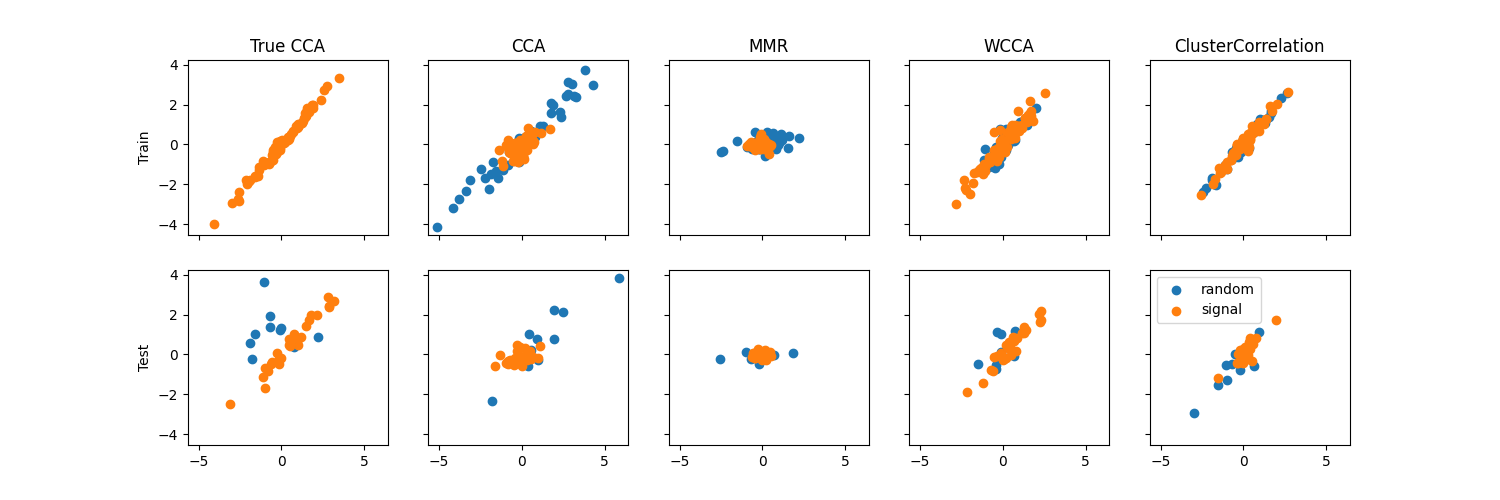
\includegraphics[width=0.9\textwidth]{chapters/sampleselection/cca/models.png}
    \caption{Plots of the first latent score for each view plotted against each other as a scatter plot. The leftmost model is trained using only the interesting data and therefore presents a ground truth}
    \label{fig:ccalatent}
\end{figure}

\begin{figure}[H] 
    \centering
    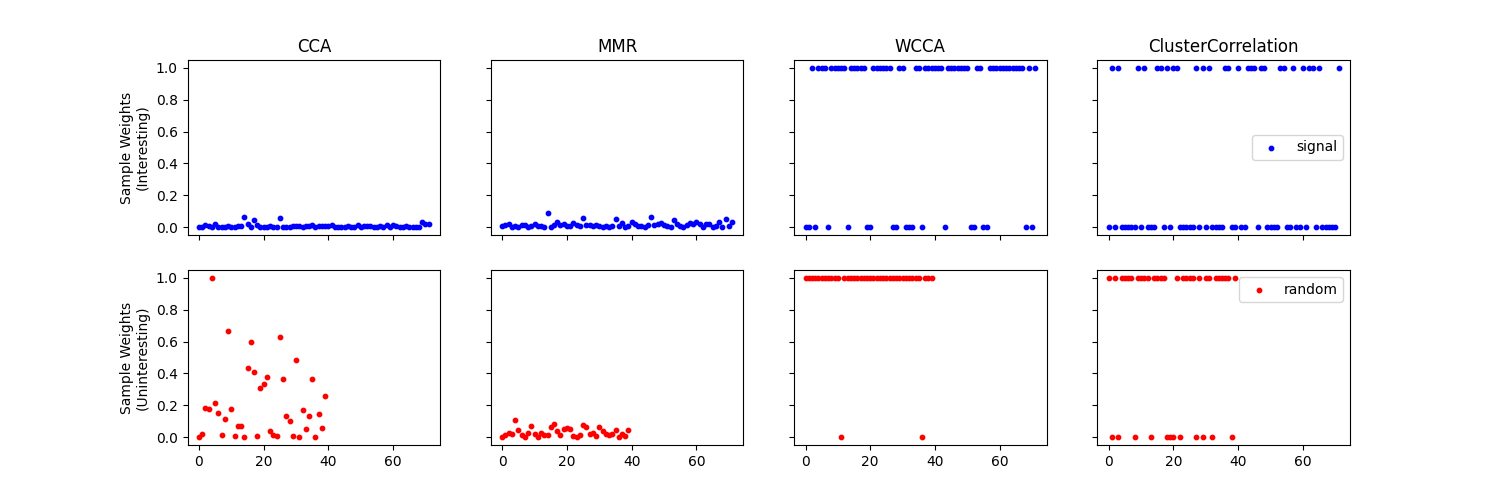
\includegraphics[width=0.9\textwidth]{chapters/sampleselection/cca/weights.png}
    \caption{Plots showing the implied sample weights by both models with the rows separating the interesting samples (top) from the uninteresting samples (bottom). An ideal model would have all samples=1 in the top row and all samples=0 in the bottom.}
    \label{fig:ccaweights}
\end{figure}

\section{Future Work}

This project remains at a somewhat exploratory stage so much of the future work will need to identify situations where these methods could be valuable.

\subsection{Application to GENFI Dataset}

This dataset has the interesting property of containing ground truth subtypes which could be used to validate any promising models. Recent work using Group Factor Analysis \cite{Ferreira2021} has shown promise extracting meaningful brain-behaviour associations using a probabilistic model and upcoming work by the same authors uses probabilistic model with sparsity over subjects. This provides a useful benchmark for our work.



\chapter{Software Contributions}\label{ch:software-contributions}

\section{Introduction}

This chapter describes major software contributions made during the course of this thesis. In particular, this chapter describes the development of the \texttt{CCA-Zoo} Python package which provides a unified interface for canonical correlation analysis (CCA) and related methods. It also briefly describes \texttt{ProxTorch}, a Pytorch compatible package containing implementations of proximal operators for use in optimisation. Finally, it describes minor contributions to the \texttt{CCA/PLS Toolkit} for Multiview Analysis of Neuroimaging data in MATLAB.

\section{Python: CCA-Zoo: A collection of regularised, Deep Learning based, Kernel, and Probabilistic CCA methods in a scikit-learn style framework}\label{sec:ccazoo}

\subsection{Statement of need}
The Python ecosystem for multiview learning currently provides a few options for implementing CCA and PLS models. scikit-learn \cite{pedregosa2011scikit} contains standard implementations of both CCA and PLS for two-view data which plug into their mature API. pyrcca \cite{bilenko2016pyrcca} contains implementations of ridge regularised and kernelized two-view CCA. The embed module of mvlearn \cite{perry2020mvlearn} is perhaps the closest relative of cca-zoo, containing implementations of ridge regularised and kernelized multi-view CCA. cca-zoo builds on the mvlearn API by providing an additional range of regularised models and in particular sparsity inducing models which have found success in multiomics. Building on the reference implementation in mvlearn, cca-zoo further provides a number of deep learning models with a modular design to enable users to supply their own choice of neural network architectures.

Standard implementations of state-of-the-art models help as benchmarks for methods development and easy application to new datasets. cca-zoo extends the existing ecosystem with a number of sparse regularised CCA models. These variations have found popularity in genetics and neuroimaging where signals are contained in a small subset of variables. With applications like these in mind, cca-zoo simplified the access to the learnt model weights to perform further analysis in the feature space. Furthermore, the modular implementations of deep CCA and its multiview variants allow the user to focus on architecture tuning. Finally, cca-zoo adds generative models including variational \cite{wang2007variational} and deep variational CCA \cite{wang2016deep} as well as higher order canonical correlation analysis with tensor \cite{kim2007tensor} and deep tensor CCA \cite{wong2021deep}.

\subsection{Implementation}
cca-zoo adopted a similar API to that used in scikit-learn. The user first instantiates a model object and its relevant hyperparameters. Next they call the model's fit() method to apply the data. After fitting, the model object contains its relevant parameters such as weights or dual coefficients (for kernel methods) which can be accessed for further analysis. For models that fit with iterative algorithms, the model may also contain information about the convergence of the objective function. After the model has been fit, its transform() method can project views into latent variables and score() can be used to measure the canonical correlations.

The deep and probabilistic models are supported by PyTorch and NumPyro respectively. Due to the size of these dependencies, these two classes of variations are not in the default installation. Instead, we provide options [deep] and [probabilistic] for users. The list bellow provides the complete collection of models along with their installation tag is provided below.

\subsection{Model List}

A complete model list at the time of publication:

\begin{center}
\begin{tabular}{|| p{0.2\textwidth}|p{0.4\textwidth}|p{0.1\textwidth}|p{0.1\textwidth} ||}
    \hline
    Model Class & Model Name & Number of Views & Install\\
    \hline \hline
    CCA & Canonical Correlation Analysis & 2 & standard\\
    \hline
    rCCA & Canonical Ridge & 2 & standard\\
    \hline
    KCCA & Kernel Canonical Correlation Analysis & 2 & standard\\
    \hline
    MCCA & Multiset Canonical Correlation Analysis & >=2 & standard\\
    \hline
    KMCCA & Kernel Multiset Canonical Correlation Analysis & >=2 & standard\\
    \hline
    GCCA & Generalized Canonical Correlation Analysis & >=2 & standard\\
    \hline
    KGCCA & Kernel Generalized Canonical Correlation Analysis & >=2 & standard\\
    \hline
    PLS & Partial Least Squares & >=2 & standard\\
    \hline
    CCA\_ALS & Canonical Correlation Analysis by Alternating Least Squares) \cite{golub1995canonical} & >=2 & standard\\
    \hline
    PLS\_ALS & Partial Least Squares by Alternating Least Squares) & >=2 & standard\\
    \hline
    PMD & Sparse CCA by Penalized Matrix Decomposition & >=2 & standard\\
    \hline
    ElasticCCA & Sparse Penalized CCA \cite{waaijenborg2008quantifying} & >=2 & standard\\
    \hline
    ParkhomenkoCCA & Sparse CCA \cite{parkhomenko2009sparse} & >=2 & standard\\
    \hline
    SCCA & Sparse Canonical Correlation Analysis by Iterative Least Squares \cite{mai2019iterative} & >=2 & standard\\
    \hline
    SCCA\_ADMM & Sparse Canonical Correlation Analysis by Altnerating Direction Method of Multipliers \cite{suo2017sparse} & >=2 & standard\\
    \hline
    SpanCCA & Sparse Diagonal Canonical Correlation Analysis \cite{asteris2016simple} & >=2 & standard\\
    \hline
    SWCCA & Sparse Weighted Canonical Correlation Analysis \cite{wenwen2018sparse} & >=2 & standard\\
    \hline
    TCCA & Tensor Canonical Correlation Analysis & >=2 & standard\\
    \hline
    KTCCA & Kernel Tensor Canonical Correlation Analysis \cite{kim2007tensor} & >=2 & standard\\
    \hline
    DCCA & Deep Canonical Correlation Analysis & >=2 & deep\\
    \hline
    DCCA\_NOI & Deep Canonical Correlation Analysis by Non-Linear Orthogonal Iterations \cite{wang2015stochastic} & >=2 & deep\\
    \hline
    DCCAE & Deep Canonically Correlated Autoencoders \cite{wang2015deep} & >=2 & deep\\
    \hline
    DTCCA & Deep Tensor Canonical Correlation Analysis & >=2 & deep\\
    \hline
    SplitAE & Split Autoencoders \cite{ngiam2011multimodal} & 2 & deep\\
    \hline
    DVCCA & Deep Variational Canonical Correlation Analysis & >=2 & deep\\
    \hline
    ProbabilisticCCA & Probabilistic Canonical Correlation Analysis & 2 & probabilistic\\
    \hline
\end{tabular}
\end{center}


\subsection{Documentation}

The package is accompanied by documentation (https://cca-zoo.readthedocs.io/en/latest/index.html) and a number of tutorial notebooks which serve as both guides to the package as well as educational resources for CCA and PLS methods.

\subsection{Conclusion}

cca-zoo fills many of the gaps in the multiview learning ecosystem in Python, including a flexible API for deep-learning based models, regularised models for high dimensional data (and in particular those that induce sparsity), and generative models.cca-zoo will therefore help researchers to apply and develop Canonical Correlation Analysis and Partial Least Squares models. We continue to welcome contributions from the community.

\subsection{Contribution}

I was the first author of two.

\section{ProxTorch}\label{sec:proxtorch}

\subsection{Introduction}

In an era where deep learning frameworks like PyTorch are the cornerstone of modern machine learning applications, the need for specialized optimization techniques is ever-growing.
While gradient-based optimization methods have been front and center in this evolution, the utility of proximal gradient descent in handling non-smooth problems remains indisputable.
However, a seamless integration of proximal operators into the PyTorch ecosystem has been noticeably missing.
`ProxTorch` emerges as a groundbreaking software library to fill this void, offering a wide array of proximal operators that are fully compatible with PyTorch and optimized for GPU computations.

\subsection{Background}

Over the years, optimization techniques have evolved to solve increasingly complex problems.
Specifically, proximal gradient descent has found applications across diverse domains like imaging, signal processing, and machine learning.
However, most existing software libraries for proximal gradient descent are either problem-specific or confined to CPU-based, numpy-compatible environments.
Meanwhile, PyTorch, a powerful deep learning framework with GPU support, lacked a dedicated library for proximal operators.
Thus, the divide between proximal optimization and mainstream deep learning frameworks like PyTorch needed to be bridged.

\subsection{Implementation}

\subsubsection{API}

`ProxTorch` presents a clean and intuitive API that allows users to easily incorporate a variety of proximal operators into their PyTorch-based projects.
It includes constraints such as L0Ball, L1Ball, L2Ball, and many others, along with regularizers like ElasticNet, GroupLasso, and Huber loss among others.
This rich collection makes it an ideal tool for both practitioners and researchers working on optimization tasks in a PyTorch setting.

\subsection{Benchmarking}

To establish its computational efficiency, `ProxTorch` was benchmarked against `Nilearn`, a numpy-based module tailored for NeuroImaging.
The focus of the benchmark was the Total Variation-L1 (TVL1) proximal operator.
Notably, `ProxTorch` outperformed `Nilearn` across different dimensions, both on CPUs and GPUs. This performance gain becomes increasingly significant with growing data dimensions, emphasizing the advantages of GPU acceleration.

\subsection{Conclusion}

`ProxTorch` serves as a pivotal advancement in the field of optimization, particularly for those operating within the PyTorch ecosystem.
It unifies the realms of proximal gradient descent and deep learning, offering a comprehensive, efficient, and GPU-compatible toolbox for tackling a wide range of optimization problems.
As such, `ProxTorch` stands as an indispensable tool for both academic research and real-world applications in optimization.





\section{MATLAB: PLS/CCA Toolkit}

This is a toolkit to incorporate standard and regularized PLS/CCA models to investigate multivariate associations between multiple modalities of data, e.g. brain imaging and behaviour or brain imaging and genetics. The toolkit includes various options for PLS/CCA models (e.g. PLS, CCA, PCA-CCA, SPLS, KCCA), statistical inference (descriptive or predictive), optimizing hyperparameters for regularized PLS/CCA as well as others (e.g. different deflation strategies).

\subsection{Features}

\begin{itemize}
    \item testing the generalizablity of the associative effects using mutiple holdouts
    \item testing the stability of models during regularization hyperparameter selection
    \item iterative calculation of associative effects, i.e. optimal regularization for each associative effect
\end{itemize}

For a discussion of the importance on pipeline choices, see Mihalik et al. 2020a.

\subsection{Contribution}

Wrote MATLAB code for the generation of simulated data with as described in chapter \ref{chap:framework}. This code is used in some of the examples in the documentation and is available to users to generate their own simulated data.




\chapter*{Thoughts and Implications}
\label{cha:discussion}

\section*{Summary of findings}

\section*{Implications}

\section*{Limitations}

\section*{Future work}

\section*{Conclusion}


% -------------------  BIBLIOGRAPHY ---------------------
\newpage
\addcontentsline{toc}{chapter}{References} % Adds References Section to Table of Contents
\printbibliography[title = {References}]


\end{document}
%  -------------------------------------------------
%  --------- The document ends from here ----------- 
%  -------------------------------------------------